% Options for packages loaded elsewhere
\PassOptionsToPackage{unicode}{hyperref}
\PassOptionsToPackage{hyphens}{url}
%
\documentclass[
  11pt,
]{article}
\usepackage{lmodern}
\usepackage{amssymb,amsmath}
\usepackage{ifxetex,ifluatex}
\ifnum 0\ifxetex 1\fi\ifluatex 1\fi=0 % if pdftex
  \usepackage[T1]{fontenc}
  \usepackage[utf8]{inputenc}
  \usepackage{textcomp} % provide euro and other symbols
\else % if luatex or xetex
  \usepackage{unicode-math}
  \defaultfontfeatures{Scale=MatchLowercase}
  \defaultfontfeatures[\rmfamily]{Ligatures=TeX,Scale=1}
\fi
% Use upquote if available, for straight quotes in verbatim environments
\IfFileExists{upquote.sty}{\usepackage{upquote}}{}
\IfFileExists{microtype.sty}{% use microtype if available
  \usepackage[]{microtype}
  \UseMicrotypeSet[protrusion]{basicmath} % disable protrusion for tt fonts
}{}
\makeatletter
\@ifundefined{KOMAClassName}{% if non-KOMA class
  \IfFileExists{parskip.sty}{%
    \usepackage{parskip}
  }{% else
    \setlength{\parindent}{0pt}
    \setlength{\parskip}{6pt plus 2pt minus 1pt}}
}{% if KOMA class
  \KOMAoptions{parskip=half}}
\makeatother
\usepackage{xcolor}
\IfFileExists{xurl.sty}{\usepackage{xurl}}{} % add URL line breaks if available
\IfFileExists{bookmark.sty}{\usepackage{bookmark}}{\usepackage{hyperref}}
\hypersetup{
  pdftitle={Data science report V2},
  pdfauthor={Antonio Malatesta; Karan Soneja; Michele D'Ambrosio},
  hidelinks,
  pdfcreator={LaTeX via pandoc}}
\urlstyle{same} % disable monospaced font for URLs
\usepackage[margin=1in]{geometry}
\usepackage{color}
\usepackage{fancyvrb}
\newcommand{\VerbBar}{|}
\newcommand{\VERB}{\Verb[commandchars=\\\{\}]}
\DefineVerbatimEnvironment{Highlighting}{Verbatim}{commandchars=\\\{\}}
% Add ',fontsize=\small' for more characters per line
\usepackage{framed}
\definecolor{shadecolor}{RGB}{248,248,248}
\newenvironment{Shaded}{\begin{snugshade}}{\end{snugshade}}
\newcommand{\AlertTok}[1]{\textcolor[rgb]{0.94,0.16,0.16}{#1}}
\newcommand{\AnnotationTok}[1]{\textcolor[rgb]{0.56,0.35,0.01}{\textbf{\textit{#1}}}}
\newcommand{\AttributeTok}[1]{\textcolor[rgb]{0.77,0.63,0.00}{#1}}
\newcommand{\BaseNTok}[1]{\textcolor[rgb]{0.00,0.00,0.81}{#1}}
\newcommand{\BuiltInTok}[1]{#1}
\newcommand{\CharTok}[1]{\textcolor[rgb]{0.31,0.60,0.02}{#1}}
\newcommand{\CommentTok}[1]{\textcolor[rgb]{0.56,0.35,0.01}{\textit{#1}}}
\newcommand{\CommentVarTok}[1]{\textcolor[rgb]{0.56,0.35,0.01}{\textbf{\textit{#1}}}}
\newcommand{\ConstantTok}[1]{\textcolor[rgb]{0.00,0.00,0.00}{#1}}
\newcommand{\ControlFlowTok}[1]{\textcolor[rgb]{0.13,0.29,0.53}{\textbf{#1}}}
\newcommand{\DataTypeTok}[1]{\textcolor[rgb]{0.13,0.29,0.53}{#1}}
\newcommand{\DecValTok}[1]{\textcolor[rgb]{0.00,0.00,0.81}{#1}}
\newcommand{\DocumentationTok}[1]{\textcolor[rgb]{0.56,0.35,0.01}{\textbf{\textit{#1}}}}
\newcommand{\ErrorTok}[1]{\textcolor[rgb]{0.64,0.00,0.00}{\textbf{#1}}}
\newcommand{\ExtensionTok}[1]{#1}
\newcommand{\FloatTok}[1]{\textcolor[rgb]{0.00,0.00,0.81}{#1}}
\newcommand{\FunctionTok}[1]{\textcolor[rgb]{0.00,0.00,0.00}{#1}}
\newcommand{\ImportTok}[1]{#1}
\newcommand{\InformationTok}[1]{\textcolor[rgb]{0.56,0.35,0.01}{\textbf{\textit{#1}}}}
\newcommand{\KeywordTok}[1]{\textcolor[rgb]{0.13,0.29,0.53}{\textbf{#1}}}
\newcommand{\NormalTok}[1]{#1}
\newcommand{\OperatorTok}[1]{\textcolor[rgb]{0.81,0.36,0.00}{\textbf{#1}}}
\newcommand{\OtherTok}[1]{\textcolor[rgb]{0.56,0.35,0.01}{#1}}
\newcommand{\PreprocessorTok}[1]{\textcolor[rgb]{0.56,0.35,0.01}{\textit{#1}}}
\newcommand{\RegionMarkerTok}[1]{#1}
\newcommand{\SpecialCharTok}[1]{\textcolor[rgb]{0.00,0.00,0.00}{#1}}
\newcommand{\SpecialStringTok}[1]{\textcolor[rgb]{0.31,0.60,0.02}{#1}}
\newcommand{\StringTok}[1]{\textcolor[rgb]{0.31,0.60,0.02}{#1}}
\newcommand{\VariableTok}[1]{\textcolor[rgb]{0.00,0.00,0.00}{#1}}
\newcommand{\VerbatimStringTok}[1]{\textcolor[rgb]{0.31,0.60,0.02}{#1}}
\newcommand{\WarningTok}[1]{\textcolor[rgb]{0.56,0.35,0.01}{\textbf{\textit{#1}}}}
\usepackage{longtable,booktabs}
% Correct order of tables after \paragraph or \subparagraph
\usepackage{etoolbox}
\makeatletter
\patchcmd\longtable{\par}{\if@noskipsec\mbox{}\fi\par}{}{}
\makeatother
% Allow footnotes in longtable head/foot
\IfFileExists{footnotehyper.sty}{\usepackage{footnotehyper}}{\usepackage{footnote}}
\makesavenoteenv{longtable}
\usepackage{graphicx,grffile}
\makeatletter
\def\maxwidth{\ifdim\Gin@nat@width>\linewidth\linewidth\else\Gin@nat@width\fi}
\def\maxheight{\ifdim\Gin@nat@height>\textheight\textheight\else\Gin@nat@height\fi}
\makeatother
% Scale images if necessary, so that they will not overflow the page
% margins by default, and it is still possible to overwrite the defaults
% using explicit options in \includegraphics[width, height, ...]{}
\setkeys{Gin}{width=\maxwidth,height=\maxheight,keepaspectratio}
% Set default figure placement to htbp
\makeatletter
\def\fps@figure{htbp}
\makeatother
\setlength{\emergencystretch}{3em} % prevent overfull lines
\providecommand{\tightlist}{%
  \setlength{\itemsep}{0pt}\setlength{\parskip}{0pt}}
\setcounter{secnumdepth}{5}
\usepackage{float}
\let\origfigure\figure
\let\endorigfigure\endfigure
\renewenvironment{figure}[1][2] {
    \expandafter\origfigure\expandafter[H]
} {
    \endorigfigure
}
\usepackage{booktabs}
\usepackage{longtable}
\usepackage{array}
\usepackage{multirow}
\usepackage{wrapfig}
\usepackage{float}
\usepackage{colortbl}
\usepackage{pdflscape}
\usepackage{tabu}
\usepackage{threeparttable}
\usepackage{threeparttablex}
\usepackage[normalem]{ulem}
\usepackage{makecell}
\usepackage{xcolor}
\usepackage[]{natbib}
\bibliographystyle{plainnat}

\title{Data science report V2}
\author{Antonio Malatesta \and Karan Soneja \and Michele D'Ambrosio}
\date{19/12/2019}

\begin{document}
\maketitle
\begin{abstract}
\emph{A short summary of the work.}
\end{abstract}

{
\setcounter{tocdepth}{3}
\tableofcontents
}
\newpage

\hypertarget{introduction}{%
\section{Introduction}\label{introduction}}

\emph{What motivates us to do this work. Touch on important finding in
literature. }

\hypertarget{data}{%
\section{Data}\label{data}}

The data used in this report consists of the stock price of some of the
10 biggest French companies.

\begin{table}[ht]
\caption:{Top ten firms in CAC40 by market cap, September 2019}
\centering
\begin{tabular}{|c|c|c|c|}
  \hline
Company & MNEMO  &  Sector  & Weight\% \\
  \hline
  TOTAL &   FP  & Oil and Gas & 9,54 \\
  LVMH &    MC  & Personal and Household Goods & 7,97 \\
  SANOFI & SAN  & Health Care & 7,54 \\
  AIRBUS & AIR  & Industrial Goods and Services &   5,47 \\
  L'OREAL   & OR  & Personal and Household Goods &  5,10 \\
  AIR LIQUIDE & AI  & Chemicals &   4,40 \\
  DANONE &  BN  & Food and Beverage & 4,14 \\
  VINCI &   DG & Construction and Materials & 3,97 \\
  BNP PARIBAS ACT.A &   BNP  & Banks & 3,95 \\
  SAFRAN & SAF  & Industrial Goods and Services & 3,72 \\
   \hline
  \end{tabular}
\end{table}

With the following code, we downloaded the daily open, high, low, close,
Volume and adjusted price of the desired stock from 2016-12-31 to
2018-12-31.

\begin{Shaded}
\begin{Highlighting}[]
\KeywordTok{getSymbols}\NormalTok{(}\StringTok{"COMPANY CODE"}\NormalTok{, }\DataTypeTok{src=}\StringTok{"yahoo"}\NormalTok{, }\DataTypeTok{from=}\StringTok{"2016-12-31"}\NormalTok{, }\DataTypeTok{to=}\StringTok{"2018-12-31"}\NormalTok{)}
\end{Highlighting}
\end{Shaded}

In some models, we also used economic and financial variables to test
whether they could increase the predictability power of the analysis.
See the following table for a detailed list of the variables we studied.

\begin{table}[H]

\caption{\label{tab:first_half}Additional economical variables}
\centering
\begin{tabular}[t]{ll}
\toprule
Economic
Factors & Source\\
\midrule
Daily interest rate & sdw.ecb.europa.eu\\
Daily Exchange rate
(EUR/USD) & exchangerates.org\\
Political Stability (yearly) & databank.worldbank.org\\
CPI Infaltion (monthly) & www.inflation.eu\\
\bottomrule
\end{tabular}
\end{table}

some text in between to have better formatting

\begin{table}[H]

\caption{\label{tab:second_half}Additional economical variables}
\centering
\begin{tabular}[t]{ll}
\toprule
Yearly Financial
Statements Variables & Source\\
\midrule
Dividend & \\
Revenue & \\
Net income & dividenmax.com\\
Basic earnings
per share & \\
Diluted earnings
per share & airbus.com\\
\addlinespace
Total assets & \\
Intangible assets & airliquide.com\\
PPE & \\
Cash & danone.com\\
Total equity & \\
\addlinespace
Non current liability & vinci.com\\
Cash flows from operating activities & \\
Net cash flows from
investing activities & invest.bnpparibas.com\\
Net cash flows from
financing activities & \\
Net cash and cash
equivalents at end of period & \\
\bottomrule
\end{tabular}
\end{table}

We gathered all the data mentioned above in one single master database
that can be found in the file ``master file.xlsx''.

\newpage

\hypertarget{technical-analysis-implementation-of-a-naive-strategy-in-r}{%
\section{Technical analysis: implementation of a naive strategy in
R}\label{technical-analysis-implementation-of-a-naive-strategy-in-r}}

\hypertarget{try-gp}{%
\subsection{try GP}\label{try-gp}}

Make an attempt to get the gp working naively using trading signal
generation with functions from above

\hypertarget{some-notes}{%
\subsection{Some notes}\label{some-notes}}

\hypertarget{some-useful-links}{%
\subsubsection{Some useful links}\label{some-useful-links}}

\begin{enumerate}
\def\labelenumi{\arabic{enumi}.}
\tightlist
\item
  A
  \href{http://www.tradinggeeks.net/2014/07/technical-analysis-with-r/}{list
  of easy TA indicators}. We have:

  \begin{itemize}
  \tightlist
  \item
    MA
  \item
    Bollinger bands
  \item
    RSI
  \item
    MACD The code is shown but not shared. The package is \{TTR\}
  \end{itemize}
\item
  A series of posts on trading

  \begin{itemize}
  \tightlist
  \item
    Attempt of
    \href{https://quantstrattrader.wordpress.com/category/portfolio-management/}{backtesting}
    in quantmod
  \item
    Read quickly
    \href{https://ntguardian.wordpress.com/2017/03/27/introduction-stock-market-data-r-1/}{part1};
    no need for the code beacuse it's in the next post. Here however a
    good tip on charting several price charts together. First Search
    \textless\textless{} Create a plot showing all series as lines;
    \textgreater\textgreater. Second, use return normalization (search
    for \textless\textless{} \#\# Loading required package: magrittr
    \textgreater\textgreater{} ). Not much more in this part.
  \item
    Then read
    \href{https://ntguardian.wordpress.com/2017/04/03/introduction-stock-market-data-r-2/}{part2}
  \end{itemize}
\end{enumerate}

\hypertarget{what-indicators-from-neftci1991}{%
\subsubsection{\texorpdfstring{what indicators (from
\citet{Neftci1991})}{what indicators (from @Neftci1991)}}\label{what-indicators-from-neftci1991}}

\begin{enumerate}
\def\labelenumi{\arabic{enumi}.}
\item
  Trend crossing methods

  \begin{itemize}
  \tightlist
  \item
    New item
  \end{itemize}
\item
  Moving average methods

  \begin{itemize}
  \tightlist
  \item
    Respect Markov times theorem
  \end{itemize}
\item
  As a sidenote, don't forget about the importance of having an exit
  strategy. (
  \href{https://ntguardian.wordpress.com/2017/04/03/introduction-stock-market-data-r-2/}{reminder
  here})
\item
  Add a
  \href{https://ntguardian.wordpress.com/2017/04/24/order-type-parameter-optimization-quantstrat/}{stop-loss
  rule}
\item
  On signals and rules,
  \href{https://statsmaths.github.io/stat395-f17/assets/final_project/amarnani.html}{here}
\item
  Don't forget to add a benchmarking stock (as the SPY for the US market
  ) to know what would have been like to have a long position on the
  market portfolio
\end{enumerate}

\newpage

\hypertarget{neural-networks}{%
\section{Neural networks}\label{neural-networks}}

Neural networks (NN) is a ``black box'' technique that finds non-linear
connections and recognize patterns between one or multiple inputs to
generate an output\footnote{(\url{https://pathmind.com/wiki/neural-network})}
. We will test a 1-input NN\footnote{(\url{http://rpubs.com/kapage/523169?fbclid=IwAR3RW_tVA_7SgCah7M0nmZL7anIL4gS_ZZ3dP_i_w8AOyQXoTMwXC_wQsoE})}
and a multiple-input NN\footnote{(\url{https://www.analyticsvidhya.com/blog/2017/09/creating-visualizing-neural-network-in-r/?fbclid=IwAR0z9tD0-WFxG3zVs8YmFaLF7RGnszbizQrhyGdyZG1-GL-D5coqBOnTiZE})}
in the attempt to predict the next-day stock price of our 5 stocks, over
a period of 30 trading days, from the 16/11/2018 to the 31/12/2018.
Based on the predictions, we will develop an investing strategy where
everyday, for the above-mentioned 30 days, we will invest all our
capital (starting at 10,000 euro) into the stock that will have the
biggest predicted increase in price the next day, according to our
model. Consequently, the next day we will sell all our stocks bought the
previous day, and invest again all our capital with the same reasoning.
In this analysis, all commission and brokerage fees are ignored.

\hypertarget{benchmark}{%
\subsection{Benchmark}\label{benchmark}}

To evaluate the performance of the NN as an investment decision-maker,
instead of using a ROC Curve, we decided to compare it with a
diversified, long-term investment strategy, where the initial capital of
10,000 euro is invested equally in the 5 stocks (2,000 euro per stock)
at the beginning of the period (16/11/2018) and all stocks are then sold
at the end of the period (31/12/2018).

\begin{table}[H]

\caption{\label{tab:benchmark2}Benchmark strategy outcome}
\centering
\resizebox{\linewidth}{!}{
\begin{tabular}[t]{llllllll}
\toprule
Dates & AIR.PA & FP.PA & MC.PA & OR.PA & SAN.PA &   & Capital\\
\midrule
16/11/2018 & 95.86 & 92.88 & 45.19 & 65.09 & 77.09 & stock price(euro) & Total budget(euro)\\
 & 2000 & 2000 & 2000 & 2000 & 2000 & amount invested(euro) & 10000\\
 & 20.86 & 21.53 & 44.25 & 30.72 & 25.94 & N. of shares bought & \\
\hline
31/12/2018 & 98.59 & 83.95 & 39.47 & 61.5 & 72.01 & stock price(euro) & Total budget(euro)\\
 & 2056.89 & 1807.72 & 1746.87 & 1889.7 & 1868.22 & value in stocks(euro) & 9369.43\\
\bottomrule
\end{tabular}}
\end{table}

As can be seen, the benchmark strategy has a return of -6\%. Clearly,
the higher the return of the NN-based investments, the more successful
the NN algorithms will be. Moreover, in case of a return lower than -6\%
(lower than the ``naive'' strategy), the NN model will be considered as
not useful in predicting stock prices.

\hypertarget{input-nn}{%
\subsection{1-input NN}\label{input-nn}}

The first NN model is a single hidden layer neural network. In this
model there is one layer of input nodes that send weighted inputs to a
subsequent layer of receiving nodes. The nnetar function in the forecast
package fits a single hidden layer neural network model to a timeseries.
The function model approach is to use lagged values of the time series
as input data, reaching to a non-linear autoregressive model. The model
takes as input the stock prices starting from the 31/12/2016 to
31/12/2018. The goal is to predict the stock prices between 16/11/2018
and 31/12/2018.

\begin{Shaded}
\begin{Highlighting}[]
\KeywordTok{library}\NormalTok{(prophet)}
\KeywordTok{library}\NormalTok{(quantmod)}
\KeywordTok{library}\NormalTok{(forecast)}
\KeywordTok{library}\NormalTok{(xlsx)}
\KeywordTok{library}\NormalTok{(tseries)}
\KeywordTok{library}\NormalTok{(timeSeries)}
\KeywordTok{library}\NormalTok{(dplyr)}
\KeywordTok{library}\NormalTok{(fGarch)}
\CommentTok{#Download the prices for the 5 stocks for the desired time frame}
\KeywordTok{getSymbols}\NormalTok{(}\StringTok{"AI.PA"}\NormalTok{, }\DataTypeTok{src=}\StringTok{"yahoo"}\NormalTok{, }\DataTypeTok{from=}\StringTok{"2016-12-31"}\NormalTok{, }\DataTypeTok{to=}\StringTok{"2018-12-31"}\NormalTok{)}
\KeywordTok{getSymbols}\NormalTok{(}\StringTok{"AIR.PA"}\NormalTok{, }\DataTypeTok{src=}\StringTok{"yahoo"}\NormalTok{, }\DataTypeTok{from=}\StringTok{"2016-12-31"}\NormalTok{, }\DataTypeTok{to=}\StringTok{"2018-12-31"}\NormalTok{)}
\KeywordTok{getSymbols}\NormalTok{(}\StringTok{"BN.PA"}\NormalTok{, }\DataTypeTok{src=}\StringTok{"yahoo"}\NormalTok{, }\DataTypeTok{from=}\StringTok{"2016-12-31"}\NormalTok{, }\DataTypeTok{to=}\StringTok{"2018-12-31"}\NormalTok{)}
\KeywordTok{getSymbols}\NormalTok{(}\StringTok{"BNP.PA"}\NormalTok{, }\DataTypeTok{src=}\StringTok{"yahoo"}\NormalTok{, }\DataTypeTok{from=}\StringTok{"2016-12-31"}\NormalTok{, }\DataTypeTok{to=}\StringTok{"2018-12-31"}\NormalTok{)}
\KeywordTok{getSymbols}\NormalTok{(}\StringTok{"DG.PA"}\NormalTok{, }\DataTypeTok{src=}\StringTok{"yahoo"}\NormalTok{, }\DataTypeTok{from=}\StringTok{"2016-12-31"}\NormalTok{, }\DataTypeTok{to=}\StringTok{"2018-12-31"}\NormalTok{)}

\NormalTok{alpha <-}\StringTok{ }\FloatTok{1.5}\OperatorTok{^}\NormalTok{(}\OperatorTok{-}\DecValTok{10}\NormalTok{)}
\end{Highlighting}
\end{Shaded}

We generate the predicted price of the 30 days for the 5 stocks with a
\texttt{for\ loop}, where the prices are predicted one at the time.

\begin{Shaded}
\begin{Highlighting}[]
\ControlFlowTok{for}\NormalTok{ (n }\ControlFlowTok{in} \DecValTok{1}\OperatorTok{:}\DecValTok{30}\NormalTok{)\{}
\NormalTok{  close_price <-}\StringTok{ }\KeywordTok{as.numeric}\NormalTok{(AIR.PA[}\DecValTok{1}\OperatorTok{:}\DecValTok{479}\OperatorTok{+}\NormalTok{n,}\StringTok{'AIR.PA.Close'}\NormalTok{])}
\CommentTok{#Hidden layers creation}
\NormalTok{  alpha <-}\StringTok{ }\FloatTok{1.5}\OperatorTok{^}\NormalTok{(}\OperatorTok{-}\DecValTok{10}\NormalTok{) }
\NormalTok{  hn <-}\StringTok{ }\KeywordTok{length}\NormalTok{(close_price)}\OperatorTok{/}\NormalTok{(alpha}\OperatorTok{*}\NormalTok{(}\KeywordTok{length}\NormalTok{(close_price)}\OperatorTok{+}\DecValTok{1}\NormalTok{))}
\CommentTok{#Fitting nnetar}
\NormalTok{  lambda <-}\StringTok{ }\KeywordTok{BoxCox.lambda}\NormalTok{(close_price)}
\NormalTok{  dnn_pred <-}\StringTok{ }\KeywordTok{nnetar}\NormalTok{(close_price, }\DataTypeTok{size=}\NormalTok{ hn, }\DataTypeTok{lambda =}\NormalTok{ lambda) }
\NormalTok{  dnn_forecast <-}\StringTok{ }\KeywordTok{forecast}\NormalTok{(dnn_pred, }\DataTypeTok{h=} \DecValTok{1}\NormalTok{, }\DataTypeTok{PI =} \OtherTok{TRUE}\NormalTok{)   }
\NormalTok{  AIR.PA.P[n] =}\StringTok{ }\NormalTok{dnn_forecast[[}\StringTok{"mean"}\NormalTok{]] }
\NormalTok{\}}

\ControlFlowTok{for}\NormalTok{ (n }\ControlFlowTok{in} \DecValTok{1}\OperatorTok{:}\DecValTok{30}\NormalTok{)\{}
\NormalTok{   close_price <-}\StringTok{ }\KeywordTok{as.numeric}\NormalTok{(BN.PA[}\DecValTok{1}\OperatorTok{:}\DecValTok{479}\OperatorTok{+}\NormalTok{n,}\StringTok{'BN.PA.Close'}\NormalTok{])}
\NormalTok{   hn <-}\StringTok{ }\KeywordTok{length}\NormalTok{(close_price)}\OperatorTok{/}\NormalTok{(alpha}\OperatorTok{*}\NormalTok{(}\KeywordTok{length}\NormalTok{(close_price)}\OperatorTok{+}\DecValTok{1}\NormalTok{))}
\NormalTok{   lambda <-}\StringTok{ }\KeywordTok{BoxCox.lambda}\NormalTok{(close_price)}
\NormalTok{   dnn_pred <-}\StringTok{ }\KeywordTok{nnetar}\NormalTok{(close_price, }\DataTypeTok{size=}\NormalTok{ hn, }\DataTypeTok{lambda =}\NormalTok{ lambda)}
\NormalTok{   dnn_forecast <-}\StringTok{ }\KeywordTok{forecast}\NormalTok{(dnn_pred, }\DataTypeTok{h=} \DecValTok{1}\NormalTok{, }\DataTypeTok{PI =} \OtherTok{TRUE}\NormalTok{)}
\NormalTok{   BN.PA.P[n] =}\StringTok{ }\NormalTok{dnn_forecast[[}\StringTok{"mean"}\NormalTok{]]}
\NormalTok{ \}}
 
 \CommentTok{#We run the same for loop above also for AI.PA, BNP.PA and DG.PA}
\end{Highlighting}
\end{Shaded}

We create a table with the predicted daily increase in price for every
stock during the 30 days. After that, we will identify the stock with
the highest predicted increase in price for every day. This will be the
stock where to invest all the capital for the day.

\begin{Shaded}
\begin{Highlighting}[]
\NormalTok{AIR.LOL <-}\StringTok{ }\NormalTok{AIR.PA.P }\OperatorTok{-}\StringTok{ }\KeywordTok{as.numeric}\NormalTok{(AIR.PA[}\DecValTok{480}\OperatorTok{:}\DecValTok{509}\NormalTok{,}\StringTok{'AIR.PA.Close'}\NormalTok{])}
\NormalTok{BN.LOL <-}\StringTok{ }\NormalTok{BN.PA.P }\OperatorTok{-}\StringTok{ }\KeywordTok{as.numeric}\NormalTok{(BN.PA[}\DecValTok{480}\OperatorTok{:}\DecValTok{509}\NormalTok{,}\StringTok{'BN.PA.Close'}\NormalTok{])}
\NormalTok{BNP.LOL <-}\StringTok{ }\NormalTok{BNP.PA.P }\OperatorTok{-}\StringTok{ }\KeywordTok{as.numeric}\NormalTok{(BNP.PA[}\DecValTok{480}\OperatorTok{:}\DecValTok{509}\NormalTok{,}\StringTok{'BNP.PA.Close'}\NormalTok{])}
\NormalTok{DG.LOL <-}\StringTok{ }\NormalTok{DG.PA.P }\OperatorTok{-}\StringTok{ }\KeywordTok{as.numeric}\NormalTok{(DG.PA[}\DecValTok{480}\OperatorTok{:}\DecValTok{509}\NormalTok{,}\StringTok{'DG.PA.Close'}\NormalTok{])}

\NormalTok{df =}\StringTok{ }\KeywordTok{data.frame}\NormalTok{(AI.LOL,AIR.LOL,BN.LOL,BNP.LOL,DG.LOL)}

\ControlFlowTok{for}\NormalTok{ (n }\ControlFlowTok{in} \DecValTok{1}\OperatorTok{:}\DecValTok{30}\NormalTok{)\{}
   \ControlFlowTok{if}\NormalTok{ (}\KeywordTok{max}\NormalTok{(df[n,]) }\OperatorTok{==}\StringTok{ }\NormalTok{df[n,}\StringTok{"AI.LOL"}\NormalTok{])\{}
\NormalTok{   AI.DIF[n] =}\StringTok{ "AI.PA"}
\NormalTok{   \} }\ControlFlowTok{else} \ControlFlowTok{if}\NormalTok{ (}\KeywordTok{max}\NormalTok{(df[n,]) }\OperatorTok{==}\StringTok{ }\NormalTok{df[n,}\StringTok{"AIR.LOL"}\NormalTok{])\{}
\NormalTok{   AI.DIF[n] =}\StringTok{ "AIR.PA"}
\NormalTok{   \} }\ControlFlowTok{else} \ControlFlowTok{if}\NormalTok{ (}\KeywordTok{max}\NormalTok{(df[n,]) }\OperatorTok{==}\StringTok{ }\NormalTok{df[n,}\StringTok{"BN.LOL"}\NormalTok{])\{}
\NormalTok{   AI.DIF[n] =}\StringTok{ "BN.PA"}
\NormalTok{   \} }\ControlFlowTok{else} \ControlFlowTok{if}\NormalTok{ (}\KeywordTok{max}\NormalTok{(df[n,]) }\OperatorTok{==}\StringTok{ }\NormalTok{df[n,}\StringTok{"BNP.LOL"}\NormalTok{])\{}
\NormalTok{   AI.DIF[n] =}\StringTok{ "BNP.PA"}
\NormalTok{   \} }\ControlFlowTok{else} \ControlFlowTok{if}\NormalTok{ (}\KeywordTok{max}\NormalTok{(df[n,]) }\OperatorTok{==}\StringTok{ }\NormalTok{df[n,}\StringTok{"DG.LOL"}\NormalTok{])\{}
\NormalTok{   AI.DIF[n] =}\StringTok{ "DG.PA"}
\NormalTok{   \}}
\NormalTok{\}}
\end{Highlighting}
\end{Shaded}

\begin{longtable}[]{@{}llllllllll@{}}
\caption{1-input NN strategy outcome}\tabularnewline
\toprule
\begin{minipage}[b]{0.05\columnwidth}\raggedright
Day\strut
\end{minipage} & \begin{minipage}[b]{0.07\columnwidth}\raggedright
Invest in\strut
\end{minipage} & \begin{minipage}[b]{0.11\columnwidth}\raggedright
date\strut
\end{minipage} & \begin{minipage}[b]{0.07\columnwidth}\raggedright
AI\strut
\end{minipage} & \begin{minipage}[b]{0.07\columnwidth}\raggedright
AIR\strut
\end{minipage} & \begin{minipage}[b]{0.07\columnwidth}\raggedright
BNP\strut
\end{minipage} & \begin{minipage}[b]{0.07\columnwidth}\raggedright
BN\strut
\end{minipage} & \begin{minipage}[b]{0.07\columnwidth}\raggedright
DG\strut
\end{minipage} & \begin{minipage}[b]{0.08\columnwidth}\raggedright
\#shares bought\strut
\end{minipage} & \begin{minipage}[b]{0.09\columnwidth}\raggedright
€ Value\strut
\end{minipage}\tabularnewline
\midrule
\endfirsthead
\toprule
\begin{minipage}[b]{0.05\columnwidth}\raggedright
Day\strut
\end{minipage} & \begin{minipage}[b]{0.07\columnwidth}\raggedright
Invest in\strut
\end{minipage} & \begin{minipage}[b]{0.11\columnwidth}\raggedright
date\strut
\end{minipage} & \begin{minipage}[b]{0.07\columnwidth}\raggedright
AI\strut
\end{minipage} & \begin{minipage}[b]{0.07\columnwidth}\raggedright
AIR\strut
\end{minipage} & \begin{minipage}[b]{0.07\columnwidth}\raggedright
BNP\strut
\end{minipage} & \begin{minipage}[b]{0.07\columnwidth}\raggedright
BN\strut
\end{minipage} & \begin{minipage}[b]{0.07\columnwidth}\raggedright
DG\strut
\end{minipage} & \begin{minipage}[b]{0.08\columnwidth}\raggedright
\#shares bought\strut
\end{minipage} & \begin{minipage}[b]{0.09\columnwidth}\raggedright
€ Value\strut
\end{minipage}\tabularnewline
\midrule
\endhead
\begin{minipage}[t]{0.05\columnwidth}\raggedright
1\strut
\end{minipage} & \begin{minipage}[t]{0.07\columnwidth}\raggedright
BNP\strut
\end{minipage} & \begin{minipage}[t]{0.11\columnwidth}\raggedright
16/11/2018\strut
\end{minipage} & \begin{minipage}[t]{0.07\columnwidth}\raggedright
95.86\strut
\end{minipage} & \begin{minipage}[t]{0.07\columnwidth}\raggedright
92.88\strut
\end{minipage} & \begin{minipage}[t]{0.07\columnwidth}\raggedright
45.19\strut
\end{minipage} & \begin{minipage}[t]{0.07\columnwidth}\raggedright
65.09\strut
\end{minipage} & \begin{minipage}[t]{0.07\columnwidth}\raggedright
77.09\strut
\end{minipage} & \begin{minipage}[t]{0.08\columnwidth}\raggedright
221.26\strut
\end{minipage} & \begin{minipage}[t]{0.09\columnwidth}\raggedright
10000\strut
\end{minipage}\tabularnewline
\begin{minipage}[t]{0.05\columnwidth}\raggedright
2\strut
\end{minipage} & \begin{minipage}[t]{0.07\columnwidth}\raggedright
BNP\strut
\end{minipage} & \begin{minipage}[t]{0.11\columnwidth}\raggedright
19/11/2018\strut
\end{minipage} & \begin{minipage}[t]{0.07\columnwidth}\raggedright
95.40\strut
\end{minipage} & \begin{minipage}[t]{0.07\columnwidth}\raggedright
92.57\strut
\end{minipage} & \begin{minipage}[t]{0.07\columnwidth}\raggedright
45.28\strut
\end{minipage} & \begin{minipage}[t]{0.07\columnwidth}\raggedright
64.70\strut
\end{minipage} & \begin{minipage}[t]{0.07\columnwidth}\raggedright
76.80\strut
\end{minipage} & \begin{minipage}[t]{0.08\columnwidth}\raggedright
221.26\strut
\end{minipage} & \begin{minipage}[t]{0.09\columnwidth}\raggedright
10019.91\strut
\end{minipage}\tabularnewline
\begin{minipage}[t]{0.05\columnwidth}\raggedright
3\strut
\end{minipage} & \begin{minipage}[t]{0.07\columnwidth}\raggedright
BNP\strut
\end{minipage} & \begin{minipage}[t]{0.11\columnwidth}\raggedright
20/11/2018\strut
\end{minipage} & \begin{minipage}[t]{0.07\columnwidth}\raggedright
93.5\strut
\end{minipage} & \begin{minipage}[t]{0.07\columnwidth}\raggedright
91.07\strut
\end{minipage} & \begin{minipage}[t]{0.07\columnwidth}\raggedright
44.30\strut
\end{minipage} & \begin{minipage}[t]{0.07\columnwidth}\raggedright
64.98\strut
\end{minipage} & \begin{minipage}[t]{0.07\columnwidth}\raggedright
76.37\strut
\end{minipage} & \begin{minipage}[t]{0.08\columnwidth}\raggedright
221.26\strut
\end{minipage} & \begin{minipage}[t]{0.09\columnwidth}\raggedright
9803.07\strut
\end{minipage}\tabularnewline
\begin{minipage}[t]{0.05\columnwidth}\raggedright
4\strut
\end{minipage} & \begin{minipage}[t]{0.07\columnwidth}\raggedright
AI\strut
\end{minipage} & \begin{minipage}[t]{0.11\columnwidth}\raggedright
21/11/2018\strut
\end{minipage} & \begin{minipage}[t]{0.07\columnwidth}\raggedright
94.22\strut
\end{minipage} & \begin{minipage}[t]{0.07\columnwidth}\raggedright
93.16\strut
\end{minipage} & \begin{minipage}[t]{0.07\columnwidth}\raggedright
44.79\strut
\end{minipage} & \begin{minipage}[t]{0.07\columnwidth}\raggedright
65.41\strut
\end{minipage} & \begin{minipage}[t]{0.07\columnwidth}\raggedright
77.01\strut
\end{minipage} & \begin{minipage}[t]{0.08\columnwidth}\raggedright
105.17\strut
\end{minipage} & \begin{minipage}[t]{0.09\columnwidth}\raggedright
9910.38\strut
\end{minipage}\tabularnewline
\begin{minipage}[t]{0.05\columnwidth}\raggedright
5\strut
\end{minipage} & \begin{minipage}[t]{0.07\columnwidth}\raggedright
AIR\strut
\end{minipage} & \begin{minipage}[t]{0.11\columnwidth}\raggedright
22/11/2018\strut
\end{minipage} & \begin{minipage}[t]{0.07\columnwidth}\raggedright
93.31\strut
\end{minipage} & \begin{minipage}[t]{0.07\columnwidth}\raggedright
92.33\strut
\end{minipage} & \begin{minipage}[t]{0.07\columnwidth}\raggedright
44.28\strut
\end{minipage} & \begin{minipage}[t]{0.07\columnwidth}\raggedright
65.27\strut
\end{minipage} & \begin{minipage}[t]{0.07\columnwidth}\raggedright
76.62\strut
\end{minipage} & \begin{minipage}[t]{0.08\columnwidth}\raggedright
106.30\strut
\end{minipage} & \begin{minipage}[t]{0.09\columnwidth}\raggedright
9814.77\strut
\end{minipage}\tabularnewline
\begin{minipage}[t]{0.05\columnwidth}\raggedright
6\strut
\end{minipage} & \begin{minipage}[t]{0.07\columnwidth}\raggedright
AI\strut
\end{minipage} & \begin{minipage}[t]{0.11\columnwidth}\raggedright
23/11/2018\strut
\end{minipage} & \begin{minipage}[t]{0.07\columnwidth}\raggedright
93.86\strut
\end{minipage} & \begin{minipage}[t]{0.07\columnwidth}\raggedright
93.41\strut
\end{minipage} & \begin{minipage}[t]{0.07\columnwidth}\raggedright
44.36\strut
\end{minipage} & \begin{minipage}[t]{0.07\columnwidth}\raggedright
65.87\strut
\end{minipage} & \begin{minipage}[t]{0.07\columnwidth}\raggedright
76.86\strut
\end{minipage} & \begin{minipage}[t]{0.08\columnwidth}\raggedright
105.78\strut
\end{minipage} & \begin{minipage}[t]{0.09\columnwidth}\raggedright
9929.57\strut
\end{minipage}\tabularnewline
\begin{minipage}[t]{0.05\columnwidth}\raggedright
7\strut
\end{minipage} & \begin{minipage}[t]{0.07\columnwidth}\raggedright
AI\strut
\end{minipage} & \begin{minipage}[t]{0.11\columnwidth}\raggedright
26/11/2018\strut
\end{minipage} & \begin{minipage}[t]{0.07\columnwidth}\raggedright
95.86\strut
\end{minipage} & \begin{minipage}[t]{0.07\columnwidth}\raggedright
93.58\strut
\end{minipage} & \begin{minipage}[t]{0.07\columnwidth}\raggedright
45.34\strut
\end{minipage} & \begin{minipage}[t]{0.07\columnwidth}\raggedright
65.82\strut
\end{minipage} & \begin{minipage}[t]{0.07\columnwidth}\raggedright
78.54\strut
\end{minipage} & \begin{minipage}[t]{0.08\columnwidth}\raggedright
105.78\strut
\end{minipage} & \begin{minipage}[t]{0.09\columnwidth}\raggedright
10141.15\strut
\end{minipage}\tabularnewline
\begin{minipage}[t]{0.05\columnwidth}\raggedright
8\strut
\end{minipage} & \begin{minipage}[t]{0.07\columnwidth}\raggedright
AIR\strut
\end{minipage} & \begin{minipage}[t]{0.11\columnwidth}\raggedright
27/11/2018\strut
\end{minipage} & \begin{minipage}[t]{0.07\columnwidth}\raggedright
94.86\strut
\end{minipage} & \begin{minipage}[t]{0.07\columnwidth}\raggedright
93.69\strut
\end{minipage} & \begin{minipage}[t]{0.07\columnwidth}\raggedright
45.08\strut
\end{minipage} & \begin{minipage}[t]{0.07\columnwidth}\raggedright
66.41\strut
\end{minipage} & \begin{minipage}[t]{0.07\columnwidth}\raggedright
78.16\strut
\end{minipage} & \begin{minipage}[t]{0.08\columnwidth}\raggedright
107.10\strut
\end{minipage} & \begin{minipage}[t]{0.09\columnwidth}\raggedright
10035.36\strut
\end{minipage}\tabularnewline
\begin{minipage}[t]{0.05\columnwidth}\raggedright
9\strut
\end{minipage} & \begin{minipage}[t]{0.07\columnwidth}\raggedright
BNP\strut
\end{minipage} & \begin{minipage}[t]{0.11\columnwidth}\raggedright
28/11/2018\strut
\end{minipage} & \begin{minipage}[t]{0.07\columnwidth}\raggedright
94.36\strut
\end{minipage} & \begin{minipage}[t]{0.07\columnwidth}\raggedright
93.5\strut
\end{minipage} & \begin{minipage}[t]{0.07\columnwidth}\raggedright
44.75\strut
\end{minipage} & \begin{minipage}[t]{0.07\columnwidth}\raggedright
65.41\strut
\end{minipage} & \begin{minipage}[t]{0.07\columnwidth}\raggedright
77.95\strut
\end{minipage} & \begin{minipage}[t]{0.08\columnwidth}\raggedright
223.75\strut
\end{minipage} & \begin{minipage}[t]{0.09\columnwidth}\raggedright
10013.94\strut
\end{minipage}\tabularnewline
\begin{minipage}[t]{0.05\columnwidth}\raggedright
10\strut
\end{minipage} & \begin{minipage}[t]{0.07\columnwidth}\raggedright
AI\strut
\end{minipage} & \begin{minipage}[t]{0.11\columnwidth}\raggedright
29/11/2018\strut
\end{minipage} & \begin{minipage}[t]{0.07\columnwidth}\raggedright
94.68\strut
\end{minipage} & \begin{minipage}[t]{0.07\columnwidth}\raggedright
94.86\strut
\end{minipage} & \begin{minipage}[t]{0.07\columnwidth}\raggedright
44.77\strut
\end{minipage} & \begin{minipage}[t]{0.07\columnwidth}\raggedright
65.54\strut
\end{minipage} & \begin{minipage}[t]{0.07\columnwidth}\raggedright
77.58\strut
\end{minipage} & \begin{minipage}[t]{0.08\columnwidth}\raggedright
105.81\strut
\end{minipage} & \begin{minipage}[t]{0.09\columnwidth}\raggedright
10018.42\strut
\end{minipage}\tabularnewline
\begin{minipage}[t]{0.05\columnwidth}\raggedright
11\strut
\end{minipage} & \begin{minipage}[t]{0.07\columnwidth}\raggedright
AI\strut
\end{minipage} & \begin{minipage}[t]{0.11\columnwidth}\raggedright
30/11/2018\strut
\end{minipage} & \begin{minipage}[t]{0.07\columnwidth}\raggedright
97.04\strut
\end{minipage} & \begin{minipage}[t]{0.07\columnwidth}\raggedright
94.62\strut
\end{minipage} & \begin{minipage}[t]{0.07\columnwidth}\raggedright
44.37\strut
\end{minipage} & \begin{minipage}[t]{0.07\columnwidth}\raggedright
66.05\strut
\end{minipage} & \begin{minipage}[t]{0.07\columnwidth}\raggedright
77.09\strut
\end{minipage} & \begin{minipage}[t]{0.08\columnwidth}\raggedright
105.81\strut
\end{minipage} & \begin{minipage}[t]{0.09\columnwidth}\raggedright
10268.51\strut
\end{minipage}\tabularnewline
\begin{minipage}[t]{0.05\columnwidth}\raggedright
12\strut
\end{minipage} & \begin{minipage}[t]{0.07\columnwidth}\raggedright
AI\strut
\end{minipage} & \begin{minipage}[t]{0.11\columnwidth}\raggedright
03/12/2018\strut
\end{minipage} & \begin{minipage}[t]{0.07\columnwidth}\raggedright
97.27\strut
\end{minipage} & \begin{minipage}[t]{0.07\columnwidth}\raggedright
95.69\strut
\end{minipage} & \begin{minipage}[t]{0.07\columnwidth}\raggedright
44.84\strut
\end{minipage} & \begin{minipage}[t]{0.07\columnwidth}\raggedright
65.41\strut
\end{minipage} & \begin{minipage}[t]{0.07\columnwidth}\raggedright
75.40\strut
\end{minipage} & \begin{minipage}[t]{0.08\columnwidth}\raggedright
105.81\strut
\end{minipage} & \begin{minipage}[t]{0.09\columnwidth}\raggedright
10292.56\strut
\end{minipage}\tabularnewline
\begin{minipage}[t]{0.05\columnwidth}\raggedright
13\strut
\end{minipage} & \begin{minipage}[t]{0.07\columnwidth}\raggedright
AI\strut
\end{minipage} & \begin{minipage}[t]{0.11\columnwidth}\raggedright
04/12/2018\strut
\end{minipage} & \begin{minipage}[t]{0.07\columnwidth}\raggedright
97.45\strut
\end{minipage} & \begin{minipage}[t]{0.07\columnwidth}\raggedright
94.26\strut
\end{minipage} & \begin{minipage}[t]{0.07\columnwidth}\raggedright
43.86\strut
\end{minipage} & \begin{minipage}[t]{0.07\columnwidth}\raggedright
65.52\strut
\end{minipage} & \begin{minipage}[t]{0.07\columnwidth}\raggedright
76.66\strut
\end{minipage} & \begin{minipage}[t]{0.08\columnwidth}\raggedright
105.81\strut
\end{minipage} & \begin{minipage}[t]{0.09\columnwidth}\raggedright
10311.81\strut
\end{minipage}\tabularnewline
\begin{minipage}[t]{0.05\columnwidth}\raggedright
14\strut
\end{minipage} & \begin{minipage}[t]{0.07\columnwidth}\raggedright
BNP\strut
\end{minipage} & \begin{minipage}[t]{0.11\columnwidth}\raggedright
05/12/2018\strut
\end{minipage} & \begin{minipage}[t]{0.07\columnwidth}\raggedright
96.45\strut
\end{minipage} & \begin{minipage}[t]{0.07\columnwidth}\raggedright
92.30\strut
\end{minipage} & \begin{minipage}[t]{0.07\columnwidth}\raggedright
43.41\strut
\end{minipage} & \begin{minipage}[t]{0.07\columnwidth}\raggedright
64.58\strut
\end{minipage} & \begin{minipage}[t]{0.07\columnwidth}\raggedright
74.66\strut
\end{minipage} & \begin{minipage}[t]{0.08\columnwidth}\raggedright
235.05\strut
\end{minipage} & \begin{minipage}[t]{0.09\columnwidth}\raggedright
10206.00\strut
\end{minipage}\tabularnewline
\begin{minipage}[t]{0.05\columnwidth}\raggedright
15\strut
\end{minipage} & \begin{minipage}[t]{0.07\columnwidth}\raggedright
DG\strut
\end{minipage} & \begin{minipage}[t]{0.11\columnwidth}\raggedright
06/12/2018\strut
\end{minipage} & \begin{minipage}[t]{0.07\columnwidth}\raggedright
94.63\strut
\end{minipage} & \begin{minipage}[t]{0.07\columnwidth}\raggedright
88.63\strut
\end{minipage} & \begin{minipage}[t]{0.07\columnwidth}\raggedright
41.78\strut
\end{minipage} & \begin{minipage}[t]{0.07\columnwidth}\raggedright
63.43\strut
\end{minipage} & \begin{minipage}[t]{0.07\columnwidth}\raggedright
70.98\strut
\end{minipage} & \begin{minipage}[t]{0.08\columnwidth}\raggedright
138.37\strut
\end{minipage} & \begin{minipage}[t]{0.09\columnwidth}\raggedright
9821.69\strut
\end{minipage}\tabularnewline
\begin{minipage}[t]{0.05\columnwidth}\raggedright
16\strut
\end{minipage} & \begin{minipage}[t]{0.07\columnwidth}\raggedright
AI\strut
\end{minipage} & \begin{minipage}[t]{0.11\columnwidth}\raggedright
07/12/2018\strut
\end{minipage} & \begin{minipage}[t]{0.07\columnwidth}\raggedright
95.86\strut
\end{minipage} & \begin{minipage}[t]{0.07\columnwidth}\raggedright
89.07\strut
\end{minipage} & \begin{minipage}[t]{0.07\columnwidth}\raggedright
41.59\strut
\end{minipage} & \begin{minipage}[t]{0.07\columnwidth}\raggedright
63.79\strut
\end{minipage} & \begin{minipage}[t]{0.07\columnwidth}\raggedright
72.68\strut
\end{minipage} & \begin{minipage}[t]{0.08\columnwidth}\raggedright
104.90\strut
\end{minipage} & \begin{minipage}[t]{0.09\columnwidth}\raggedright
10056.92\strut
\end{minipage}\tabularnewline
\begin{minipage}[t]{0.05\columnwidth}\raggedright
17\strut
\end{minipage} & \begin{minipage}[t]{0.07\columnwidth}\raggedright
DG\strut
\end{minipage} & \begin{minipage}[t]{0.11\columnwidth}\raggedright
10/12/2018\strut
\end{minipage} & \begin{minipage}[t]{0.07\columnwidth}\raggedright
95.77\strut
\end{minipage} & \begin{minipage}[t]{0.07\columnwidth}\raggedright
87.48\strut
\end{minipage} & \begin{minipage}[t]{0.07\columnwidth}\raggedright
40.40\strut
\end{minipage} & \begin{minipage}[t]{0.07\columnwidth}\raggedright
62.97\strut
\end{minipage} & \begin{minipage}[t]{0.07\columnwidth}\raggedright
71.66\strut
\end{minipage} & \begin{minipage}[t]{0.08\columnwidth}\raggedright
140.20\strut
\end{minipage} & \begin{minipage}[t]{0.09\columnwidth}\raggedright
10047.38\strut
\end{minipage}\tabularnewline
\begin{minipage}[t]{0.05\columnwidth}\raggedright
18\strut
\end{minipage} & \begin{minipage}[t]{0.07\columnwidth}\raggedright
DG\strut
\end{minipage} & \begin{minipage}[t]{0.11\columnwidth}\raggedright
11/12/2018\strut
\end{minipage} & \begin{minipage}[t]{0.07\columnwidth}\raggedright
96.45\strut
\end{minipage} & \begin{minipage}[t]{0.07\columnwidth}\raggedright
88.59\strut
\end{minipage} & \begin{minipage}[t]{0.07\columnwidth}\raggedright
40.68\strut
\end{minipage} & \begin{minipage}[t]{0.07\columnwidth}\raggedright
62.81\strut
\end{minipage} & \begin{minipage}[t]{0.07\columnwidth}\raggedright
73.69\strut
\end{minipage} & \begin{minipage}[t]{0.08\columnwidth}\raggedright
140.20\strut
\end{minipage} & \begin{minipage}[t]{0.09\columnwidth}\raggedright
10333.41\strut
\end{minipage}\tabularnewline
\begin{minipage}[t]{0.05\columnwidth}\raggedright
19\strut
\end{minipage} & \begin{minipage}[t]{0.07\columnwidth}\raggedright
AI\strut
\end{minipage} & \begin{minipage}[t]{0.11\columnwidth}\raggedright
12/12/2018\strut
\end{minipage} & \begin{minipage}[t]{0.07\columnwidth}\raggedright
97.54\strut
\end{minipage} & \begin{minipage}[t]{0.07\columnwidth}\raggedright
91.48\strut
\end{minipage} & \begin{minipage}[t]{0.07\columnwidth}\raggedright
41.90\strut
\end{minipage} & \begin{minipage}[t]{0.07\columnwidth}\raggedright
64.12\strut
\end{minipage} & \begin{minipage}[t]{0.07\columnwidth}\raggedright
74.77\strut
\end{minipage} & \begin{minipage}[t]{0.08\columnwidth}\raggedright
107.48\strut
\end{minipage} & \begin{minipage}[t]{0.09\columnwidth}\raggedright
10484.84\strut
\end{minipage}\tabularnewline
\begin{minipage}[t]{0.05\columnwidth}\raggedright
20\strut
\end{minipage} & \begin{minipage}[t]{0.07\columnwidth}\raggedright
BN\strut
\end{minipage} & \begin{minipage}[t]{0.11\columnwidth}\raggedright
13/12/2018\strut
\end{minipage} & \begin{minipage}[t]{0.07\columnwidth}\raggedright
97.63\strut
\end{minipage} & \begin{minipage}[t]{0.07\columnwidth}\raggedright
89.97\strut
\end{minipage} & \begin{minipage}[t]{0.07\columnwidth}\raggedright
42.18\strut
\end{minipage} & \begin{minipage}[t]{0.07\columnwidth}\raggedright
64.32\strut
\end{minipage} & \begin{minipage}[t]{0.07\columnwidth}\raggedright
74.5\strut
\end{minipage} & \begin{minipage}[t]{0.08\columnwidth}\raggedright
163.16\strut
\end{minipage} & \begin{minipage}[t]{0.09\columnwidth}\raggedright
10494.62\strut
\end{minipage}\tabularnewline
\begin{minipage}[t]{0.05\columnwidth}\raggedright
21\strut
\end{minipage} & \begin{minipage}[t]{0.07\columnwidth}\raggedright
BNP\strut
\end{minipage} & \begin{minipage}[t]{0.11\columnwidth}\raggedright
14/12/2018\strut
\end{minipage} & \begin{minipage}[t]{0.07\columnwidth}\raggedright
97.45\strut
\end{minipage} & \begin{minipage}[t]{0.07\columnwidth}\raggedright
88.66\strut
\end{minipage} & \begin{minipage}[t]{0.07\columnwidth}\raggedright
41.59\strut
\end{minipage} & \begin{minipage}[t]{0.07\columnwidth}\raggedright
64.08\strut
\end{minipage} & \begin{minipage}[t]{0.07\columnwidth}\raggedright
73.51\strut
\end{minipage} & \begin{minipage}[t]{0.08\columnwidth}\raggedright
251.36\strut
\end{minipage} & \begin{minipage}[t]{0.09\columnwidth}\raggedright
10455.46\strut
\end{minipage}\tabularnewline
\begin{minipage}[t]{0.05\columnwidth}\raggedright
22\strut
\end{minipage} & \begin{minipage}[t]{0.07\columnwidth}\raggedright
DG\strut
\end{minipage} & \begin{minipage}[t]{0.11\columnwidth}\raggedright
17/12/2018\strut
\end{minipage} & \begin{minipage}[t]{0.07\columnwidth}\raggedright
96.68\strut
\end{minipage} & \begin{minipage}[t]{0.07\columnwidth}\raggedright
87.65\strut
\end{minipage} & \begin{minipage}[t]{0.07\columnwidth}\raggedright
40.58\strut
\end{minipage} & \begin{minipage}[t]{0.07\columnwidth}\raggedright
63.23\strut
\end{minipage} & \begin{minipage}[t]{0.07\columnwidth}\raggedright
72.36\strut
\end{minipage} & \begin{minipage}[t]{0.08\columnwidth}\raggedright
140.96\strut
\end{minipage} & \begin{minipage}[t]{0.09\columnwidth}\raggedright
10200.32\strut
\end{minipage}\tabularnewline
\begin{minipage}[t]{0.05\columnwidth}\raggedright
23\strut
\end{minipage} & \begin{minipage}[t]{0.07\columnwidth}\raggedright
DG\strut
\end{minipage} & \begin{minipage}[t]{0.11\columnwidth}\raggedright
18/12/2018\strut
\end{minipage} & \begin{minipage}[t]{0.07\columnwidth}\raggedright
95.68\strut
\end{minipage} & \begin{minipage}[t]{0.07\columnwidth}\raggedright
88.65\strut
\end{minipage} & \begin{minipage}[t]{0.07\columnwidth}\raggedright
40.55\strut
\end{minipage} & \begin{minipage}[t]{0.07\columnwidth}\raggedright
62.68\strut
\end{minipage} & \begin{minipage}[t]{0.07\columnwidth}\raggedright
71.33\strut
\end{minipage} & \begin{minipage}[t]{0.08\columnwidth}\raggedright
140.96\strut
\end{minipage} & \begin{minipage}[t]{0.09\columnwidth}\raggedright
10056.54\strut
\end{minipage}\tabularnewline
\begin{minipage}[t]{0.05\columnwidth}\raggedright
24\strut
\end{minipage} & \begin{minipage}[t]{0.07\columnwidth}\raggedright
AI\strut
\end{minipage} & \begin{minipage}[t]{0.11\columnwidth}\raggedright
19/12/2018\strut
\end{minipage} & \begin{minipage}[t]{0.07\columnwidth}\raggedright
97.86\strut
\end{minipage} & \begin{minipage}[t]{0.07\columnwidth}\raggedright
87.19\strut
\end{minipage} & \begin{minipage}[t]{0.07\columnwidth}\raggedright
40.88\strut
\end{minipage} & \begin{minipage}[t]{0.07\columnwidth}\raggedright
62.82\strut
\end{minipage} & \begin{minipage}[t]{0.07\columnwidth}\raggedright
71.59\strut
\end{minipage} & \begin{minipage}[t]{0.08\columnwidth}\raggedright
103.13\strut
\end{minipage} & \begin{minipage}[t]{0.09\columnwidth}\raggedright
10093.19\strut
\end{minipage}\tabularnewline
\begin{minipage}[t]{0.05\columnwidth}\raggedright
25\strut
\end{minipage} & \begin{minipage}[t]{0.07\columnwidth}\raggedright
DG\strut
\end{minipage} & \begin{minipage}[t]{0.11\columnwidth}\raggedright
20/12/2018\strut
\end{minipage} & \begin{minipage}[t]{0.07\columnwidth}\raggedright
97.09\strut
\end{minipage} & \begin{minipage}[t]{0.07\columnwidth}\raggedright
83.33\strut
\end{minipage} & \begin{minipage}[t]{0.07\columnwidth}\raggedright
39.40\strut
\end{minipage} & \begin{minipage}[t]{0.07\columnwidth}\raggedright
62.25\strut
\end{minipage} & \begin{minipage}[t]{0.07\columnwidth}\raggedright
71.41\strut
\end{minipage} & \begin{minipage}[t]{0.08\columnwidth}\raggedright
140.20\strut
\end{minipage} & \begin{minipage}[t]{0.09\columnwidth}\raggedright
10013.50\strut
\end{minipage}\tabularnewline
\begin{minipage}[t]{0.05\columnwidth}\raggedright
26\strut
\end{minipage} & \begin{minipage}[t]{0.07\columnwidth}\raggedright
AI\strut
\end{minipage} & \begin{minipage}[t]{0.11\columnwidth}\raggedright
21/12/2018\strut
\end{minipage} & \begin{minipage}[t]{0.07\columnwidth}\raggedright
97.81\strut
\end{minipage} & \begin{minipage}[t]{0.07\columnwidth}\raggedright
83.09\strut
\end{minipage} & \begin{minipage}[t]{0.07\columnwidth}\raggedright
39.5\strut
\end{minipage} & \begin{minipage}[t]{0.07\columnwidth}\raggedright
62.23\strut
\end{minipage} & \begin{minipage}[t]{0.07\columnwidth}\raggedright
71.41\strut
\end{minipage} & \begin{minipage}[t]{0.08\columnwidth}\raggedright
102.36\strut
\end{minipage} & \begin{minipage}[t]{0.09\columnwidth}\raggedright
10013.50\strut
\end{minipage}\tabularnewline
\begin{minipage}[t]{0.05\columnwidth}\raggedright
27\strut
\end{minipage} & \begin{minipage}[t]{0.07\columnwidth}\raggedright
AIR\strut
\end{minipage} & \begin{minipage}[t]{0.11\columnwidth}\raggedright
24/12/2018\strut
\end{minipage} & \begin{minipage}[t]{0.07\columnwidth}\raggedright
97.09\strut
\end{minipage} & \begin{minipage}[t]{0.07\columnwidth}\raggedright
81.62\strut
\end{minipage} & \begin{minipage}[t]{0.07\columnwidth}\raggedright
38.79\strut
\end{minipage} & \begin{minipage}[t]{0.07\columnwidth}\raggedright
61.61\strut
\end{minipage} & \begin{minipage}[t]{0.07\columnwidth}\raggedright
70.5\strut
\end{minipage} & \begin{minipage}[t]{0.08\columnwidth}\raggedright
121.75\strut
\end{minipage} & \begin{minipage}[t]{0.09\columnwidth}\raggedright
9939.04\strut
\end{minipage}\tabularnewline
\begin{minipage}[t]{0.05\columnwidth}\raggedright
28\strut
\end{minipage} & \begin{minipage}[t]{0.07\columnwidth}\raggedright
AIR\strut
\end{minipage} & \begin{minipage}[t]{0.11\columnwidth}\raggedright
27/12/2018\strut
\end{minipage} & \begin{minipage}[t]{0.07\columnwidth}\raggedright
95.31\strut
\end{minipage} & \begin{minipage}[t]{0.07\columnwidth}\raggedright
82.09\strut
\end{minipage} & \begin{minipage}[t]{0.07\columnwidth}\raggedright
38.54\strut
\end{minipage} & \begin{minipage}[t]{0.07\columnwidth}\raggedright
60.27\strut
\end{minipage} & \begin{minipage}[t]{0.07\columnwidth}\raggedright
70.63\strut
\end{minipage} & \begin{minipage}[t]{0.08\columnwidth}\raggedright
121.75\strut
\end{minipage} & \begin{minipage}[t]{0.09\columnwidth}\raggedright
9996.27\strut
\end{minipage}\tabularnewline
\begin{minipage}[t]{0.05\columnwidth}\raggedright
29\strut
\end{minipage} & \begin{minipage}[t]{0.07\columnwidth}\raggedright
AI\strut
\end{minipage} & \begin{minipage}[t]{0.11\columnwidth}\raggedright
28/12/2018\strut
\end{minipage} & \begin{minipage}[t]{0.07\columnwidth}\raggedright
96.59\strut
\end{minipage} & \begin{minipage}[t]{0.07\columnwidth}\raggedright
83.76\strut
\end{minipage} & \begin{minipage}[t]{0.07\columnwidth}\raggedright
39.37\strut
\end{minipage} & \begin{minipage}[t]{0.07\columnwidth}\raggedright
60.66\strut
\end{minipage} & \begin{minipage}[t]{0.07\columnwidth}\raggedright
71.95\strut
\end{minipage} & \begin{minipage}[t]{0.08\columnwidth}\raggedright
105.58\strut
\end{minipage} & \begin{minipage}[t]{0.09\columnwidth}\raggedright
10198.39\strut
\end{minipage}\tabularnewline
\begin{minipage}[t]{0.05\columnwidth}\raggedright
30\strut
\end{minipage} & \begin{minipage}[t]{0.07\columnwidth}\raggedright
AI\strut
\end{minipage} & \begin{minipage}[t]{0.11\columnwidth}\raggedright
31/12/2018\strut
\end{minipage} & \begin{minipage}[t]{0.07\columnwidth}\raggedright
98.59\strut
\end{minipage} & \begin{minipage}[t]{0.07\columnwidth}\raggedright
83.95\strut
\end{minipage} & \begin{minipage}[t]{0.07\columnwidth}\raggedright
39.47\strut
\end{minipage} & \begin{minipage}[t]{0.07\columnwidth}\raggedright
61.50\strut
\end{minipage} & \begin{minipage}[t]{0.07\columnwidth}\raggedright
72.01\strut
\end{minipage} & \begin{minipage}[t]{0.08\columnwidth}\raggedright
\strut
\end{minipage} & \begin{minipage}[t]{0.09\columnwidth}\raggedright
10409.55\strut
\end{minipage}\tabularnewline
\bottomrule
\end{longtable}

\hypertarget{evaluation-of-1-input-nn}{%
\subsubsection{Evaluation of 1-input
NN}\label{evaluation-of-1-input-nn}}

As can be seen, the investment strategy based on the 1-input NN has a
return of +4\%, which is an extremely good result considering the
benchmark strategy return of -6\%. This implies that, even though all
the 5 stocks had negative performances during the time frame, the NN
successfully identified the right stock at the right time, leading to a
positive return.

\hypertarget{multiple-input-nn}{%
\subsection{Multiple-input NN}\label{multiple-input-nn}}

The second NN model uses the neuralnet library for the analysis. It has
3 neurons in its hidden layer and the weights are calculated using a
back propagation algorithm. The model takes several inputs that for
simpliticy have been coded according to the following table:

\begin{longtable}[]{@{}llllll@{}}
\caption{Variables coding}\tabularnewline
\toprule
\begin{minipage}[b]{0.16\columnwidth}\raggedright
Variable\strut
\end{minipage} & \begin{minipage}[b]{0.09\columnwidth}\raggedright
Identifier\strut
\end{minipage} & \begin{minipage}[b]{0.19\columnwidth}\raggedright
Variable\strut
\end{minipage} & \begin{minipage}[b]{0.09\columnwidth}\raggedright
Identifier\strut
\end{minipage} & \begin{minipage}[b]{0.21\columnwidth}\raggedright
Variable\strut
\end{minipage} & \begin{minipage}[b]{0.09\columnwidth}\raggedright
Identifier\strut
\end{minipage}\tabularnewline
\midrule
\endfirsthead
\toprule
\begin{minipage}[b]{0.16\columnwidth}\raggedright
Variable\strut
\end{minipage} & \begin{minipage}[b]{0.09\columnwidth}\raggedright
Identifier\strut
\end{minipage} & \begin{minipage}[b]{0.19\columnwidth}\raggedright
Variable\strut
\end{minipage} & \begin{minipage}[b]{0.09\columnwidth}\raggedright
Identifier\strut
\end{minipage} & \begin{minipage}[b]{0.21\columnwidth}\raggedright
Variable\strut
\end{minipage} & \begin{minipage}[b]{0.09\columnwidth}\raggedright
Identifier\strut
\end{minipage}\tabularnewline
\midrule
\endhead
\begin{minipage}[t]{0.16\columnwidth}\raggedright
Close price\strut
\end{minipage} & \begin{minipage}[t]{0.09\columnwidth}\raggedright
A1\strut
\end{minipage} & \begin{minipage}[t]{0.19\columnwidth}\raggedright
CPI monthly inflation\strut
\end{minipage} & \begin{minipage}[t]{0.09\columnwidth}\raggedright
A10\strut
\end{minipage} & \begin{minipage}[t]{0.21\columnwidth}\raggedright
PPE\strut
\end{minipage} & \begin{minipage}[t]{0.09\columnwidth}\raggedright
A18\strut
\end{minipage}\tabularnewline
\begin{minipage}[t]{0.16\columnwidth}\raggedright
Open price\strut
\end{minipage} & \begin{minipage}[t]{0.09\columnwidth}\raggedright
A2\strut
\end{minipage} & \begin{minipage}[t]{0.19\columnwidth}\raggedright
Dividend\strut
\end{minipage} & \begin{minipage}[t]{0.09\columnwidth}\raggedright
A11\strut
\end{minipage} & \begin{minipage}[t]{0.21\columnwidth}\raggedright
Cash\strut
\end{minipage} & \begin{minipage}[t]{0.09\columnwidth}\raggedright
A19\strut
\end{minipage}\tabularnewline
\begin{minipage}[t]{0.16\columnwidth}\raggedright
High price\strut
\end{minipage} & \begin{minipage}[t]{0.09\columnwidth}\raggedright
A3\strut
\end{minipage} & \begin{minipage}[t]{0.19\columnwidth}\raggedright
Revenue\strut
\end{minipage} & \begin{minipage}[t]{0.09\columnwidth}\raggedright
A12\strut
\end{minipage} & \begin{minipage}[t]{0.21\columnwidth}\raggedright
Total equity\strut
\end{minipage} & \begin{minipage}[t]{0.09\columnwidth}\raggedright
A20\strut
\end{minipage}\tabularnewline
\begin{minipage}[t]{0.16\columnwidth}\raggedright
Low price\strut
\end{minipage} & \begin{minipage}[t]{0.09\columnwidth}\raggedright
A4\strut
\end{minipage} & \begin{minipage}[t]{0.19\columnwidth}\raggedright
Net Income\strut
\end{minipage} & \begin{minipage}[t]{0.09\columnwidth}\raggedright
A13\strut
\end{minipage} & \begin{minipage}[t]{0.21\columnwidth}\raggedright
Non current liability\strut
\end{minipage} & \begin{minipage}[t]{0.09\columnwidth}\raggedright
A21\strut
\end{minipage}\tabularnewline
\begin{minipage}[t]{0.16\columnwidth}\raggedright
Volume\strut
\end{minipage} & \begin{minipage}[t]{0.09\columnwidth}\raggedright
A5\strut
\end{minipage} & \begin{minipage}[t]{0.19\columnwidth}\raggedright
Basic earnings per share\strut
\end{minipage} & \begin{minipage}[t]{0.09\columnwidth}\raggedright
A14\strut
\end{minipage} & \begin{minipage}[t]{0.21\columnwidth}\raggedright
Cash flows (used in)/from operating activities\strut
\end{minipage} & \begin{minipage}[t]{0.09\columnwidth}\raggedright
A22\strut
\end{minipage}\tabularnewline
\begin{minipage}[t]{0.16\columnwidth}\raggedright
Adjusted price\strut
\end{minipage} & \begin{minipage}[t]{0.09\columnwidth}\raggedright
A6\strut
\end{minipage} & \begin{minipage}[t]{0.19\columnwidth}\raggedright
Diluted earnings per share\strut
\end{minipage} & \begin{minipage}[t]{0.09\columnwidth}\raggedright
A15\strut
\end{minipage} & \begin{minipage}[t]{0.21\columnwidth}\raggedright
Net cash flows (used in)/from investing activities\strut
\end{minipage} & \begin{minipage}[t]{0.09\columnwidth}\raggedright
A23\strut
\end{minipage}\tabularnewline
\begin{minipage}[t]{0.16\columnwidth}\raggedright
Interest rate\strut
\end{minipage} & \begin{minipage}[t]{0.09\columnwidth}\raggedright
A7\strut
\end{minipage} & \begin{minipage}[t]{0.19\columnwidth}\raggedright
Total assets\strut
\end{minipage} & \begin{minipage}[t]{0.09\columnwidth}\raggedright
A16\strut
\end{minipage} & \begin{minipage}[t]{0.21\columnwidth}\raggedright
Net cash flows (used in)/from financing activities\strut
\end{minipage} & \begin{minipage}[t]{0.09\columnwidth}\raggedright
A24\strut
\end{minipage}\tabularnewline
\begin{minipage}[t]{0.16\columnwidth}\raggedright
Exchange rate (1 USD)\strut
\end{minipage} & \begin{minipage}[t]{0.09\columnwidth}\raggedright
A8\strut
\end{minipage} & \begin{minipage}[t]{0.19\columnwidth}\raggedright
Intangible assets\strut
\end{minipage} & \begin{minipage}[t]{0.09\columnwidth}\raggedright
A17\strut
\end{minipage} & \begin{minipage}[t]{0.21\columnwidth}\raggedright
Net cash and cash equivalents at end of period\strut
\end{minipage} & \begin{minipage}[t]{0.09\columnwidth}\raggedright
A25\strut
\end{minipage}\tabularnewline
\begin{minipage}[t]{0.16\columnwidth}\raggedright
Political stability\strut
\end{minipage} & \begin{minipage}[t]{0.09\columnwidth}\raggedright
A9\strut
\end{minipage} & \begin{minipage}[t]{0.19\columnwidth}\raggedright
\strut
\end{minipage} & \begin{minipage}[t]{0.09\columnwidth}\raggedright
\strut
\end{minipage} & \begin{minipage}[t]{0.21\columnwidth}\raggedright
\strut
\end{minipage} & \begin{minipage}[t]{0.09\columnwidth}\raggedright
\strut
\end{minipage}\tabularnewline
\bottomrule
\end{longtable}

The goal is always to predict stock prices of the 30 days, hoping that
the inclusion of additional variables like high price, low price,
inflation and financial statements data will provide more accurate
predictions.

\begin{Shaded}
\begin{Highlighting}[]
\CommentTok{#Download "AI1.csv" "AIR1.csv" "BN1.csv" "BNP1.csv" }
\CommentTok{#Download "DG1.csv" "PREDICTION SIMPLE.xlsx"}
\KeywordTok{library}\NormalTok{(readr)}
\NormalTok{AI1 <-}\StringTok{ }\KeywordTok{read_csv2}\NormalTok{(}\StringTok{"D:/2017-2018/data_analysis/technical_analysis/report/AI1.csv"}\NormalTok{)}
\NormalTok{data <-}\StringTok{ }\NormalTok{AI1[, }\KeywordTok{c}\NormalTok{(}\DecValTok{2}\OperatorTok{:}\DecValTok{26}\NormalTok{)]}
\KeywordTok{View}\NormalTok{(data)}
\CommentTok{#we take all the data frame as training data to predict the next-day stock price}
\NormalTok{datatrain =}\StringTok{ }\NormalTok{data[ }\DecValTok{1}\OperatorTok{:}\DecValTok{1531}\NormalTok{, ]}
\NormalTok{datatest =}\StringTok{ }\NormalTok{data[ }\DecValTok{1532}\NormalTok{, ]}
\CommentTok{#we normalize the values to avoid results based only on the disporportionate}
\CommentTok{#size of certain inputs}
\NormalTok{max =}\StringTok{ }\KeywordTok{apply}\NormalTok{(data , }\DecValTok{2}\NormalTok{ , max)}
\NormalTok{min =}\StringTok{ }\KeywordTok{apply}\NormalTok{(data, }\DecValTok{2}\NormalTok{ , min)}
\NormalTok{scaled =}\StringTok{ }\KeywordTok{as.data.frame}\NormalTok{(}\KeywordTok{scale}\NormalTok{(data, }\DataTypeTok{center =}\NormalTok{ min, }\DataTypeTok{scale =}\NormalTok{ max }\OperatorTok{-}\StringTok{ }\NormalTok{min))}
\CommentTok{# install library}
\KeywordTok{install.packages}\NormalTok{(}\StringTok{"neuralnet "}\NormalTok{)}
\CommentTok{#load library}
\KeywordTok{library}\NormalTok{(neuralnet)}
\CommentTok{# creating training and test set}
\CommentTok{# the test set will be the closing price of a single day}
\CommentTok{# the training set will be all the data of the days before the day of the test set}
\NormalTok{trainNN =}\StringTok{ }\NormalTok{scaled[}\DecValTok{1}\OperatorTok{:}\DecValTok{1531}\NormalTok{ , ]}
\NormalTok{testNN =}\StringTok{ }\NormalTok{scaled[}\DecValTok{1532}\NormalTok{ , ] }
\end{Highlighting}
\end{Shaded}

We want to predict every next day price for the 5 stocks. But first, we
want to check weather the the model gives more accurate results with or
without the financial statement data as inputs.

\begin{Shaded}
\begin{Highlighting}[]
\CommentTok{# fit neural network}
\KeywordTok{set.seed}\NormalTok{(}\DecValTok{2}\NormalTok{)}
\CommentTok{# Develop a NN model with tomorrow closing price as output and}
\CommentTok{# all the other variables (taken today) as input}
\NormalTok{NN =}\StringTok{ }\KeywordTok{neuralnet}\NormalTok{( A1 }\OperatorTok{~}\StringTok{ }\NormalTok{A2 }\OperatorTok{+}\StringTok{ }\NormalTok{A3 }\OperatorTok{+}\StringTok{ }\NormalTok{A4 }\OperatorTok{+}\StringTok{ }\NormalTok{A5 }\OperatorTok{+}\StringTok{ }\NormalTok{A6 }\OperatorTok{+}\StringTok{ }\NormalTok{A7 }\OperatorTok{+}\StringTok{ }\NormalTok{A8 }\OperatorTok{+}\StringTok{ }\NormalTok{A9 }\OperatorTok{+}\StringTok{ }\NormalTok{A10}
\OperatorTok{+}\StringTok{ }\NormalTok{A11 }\OperatorTok{+}\StringTok{ }\NormalTok{A12 }\OperatorTok{+}\StringTok{ }\NormalTok{A13 }\OperatorTok{+}\StringTok{ }\NormalTok{A14 }\OperatorTok{+}\StringTok{ }\NormalTok{A15 }\OperatorTok{+}\StringTok{ }\NormalTok{A16 }\OperatorTok{+}\StringTok{ }\NormalTok{A17 }\OperatorTok{+}\StringTok{ }\NormalTok{A18 }\OperatorTok{+}\StringTok{ }\NormalTok{A19 }\OperatorTok{+}\StringTok{ }\NormalTok{A20 }\OperatorTok{+}\StringTok{ }\NormalTok{A21}
\OperatorTok{+}\StringTok{ }\NormalTok{A22 }\OperatorTok{+}\StringTok{ }\NormalTok{A23 }\OperatorTok{+}\StringTok{ }\NormalTok{A24 }\OperatorTok{+}\StringTok{ }\NormalTok{A25, trainNN, }\DataTypeTok{hidden =} \DecValTok{3}\NormalTok{ , }\DataTypeTok{linear.output =}\NormalTok{ T ) }
\CommentTok{# plot neural network}
\KeywordTok{plot}\NormalTok{(NN)}
\end{Highlighting}
\end{Shaded}

In the image below we can see a graphical representation of the neuronal
net: It has 3 neurons in its hidden layer. The black lines show the
connections with weights. The weights are calculated using a back
propagation algorithm. The blue line displays the bias term.

\begin{figure}
\centering
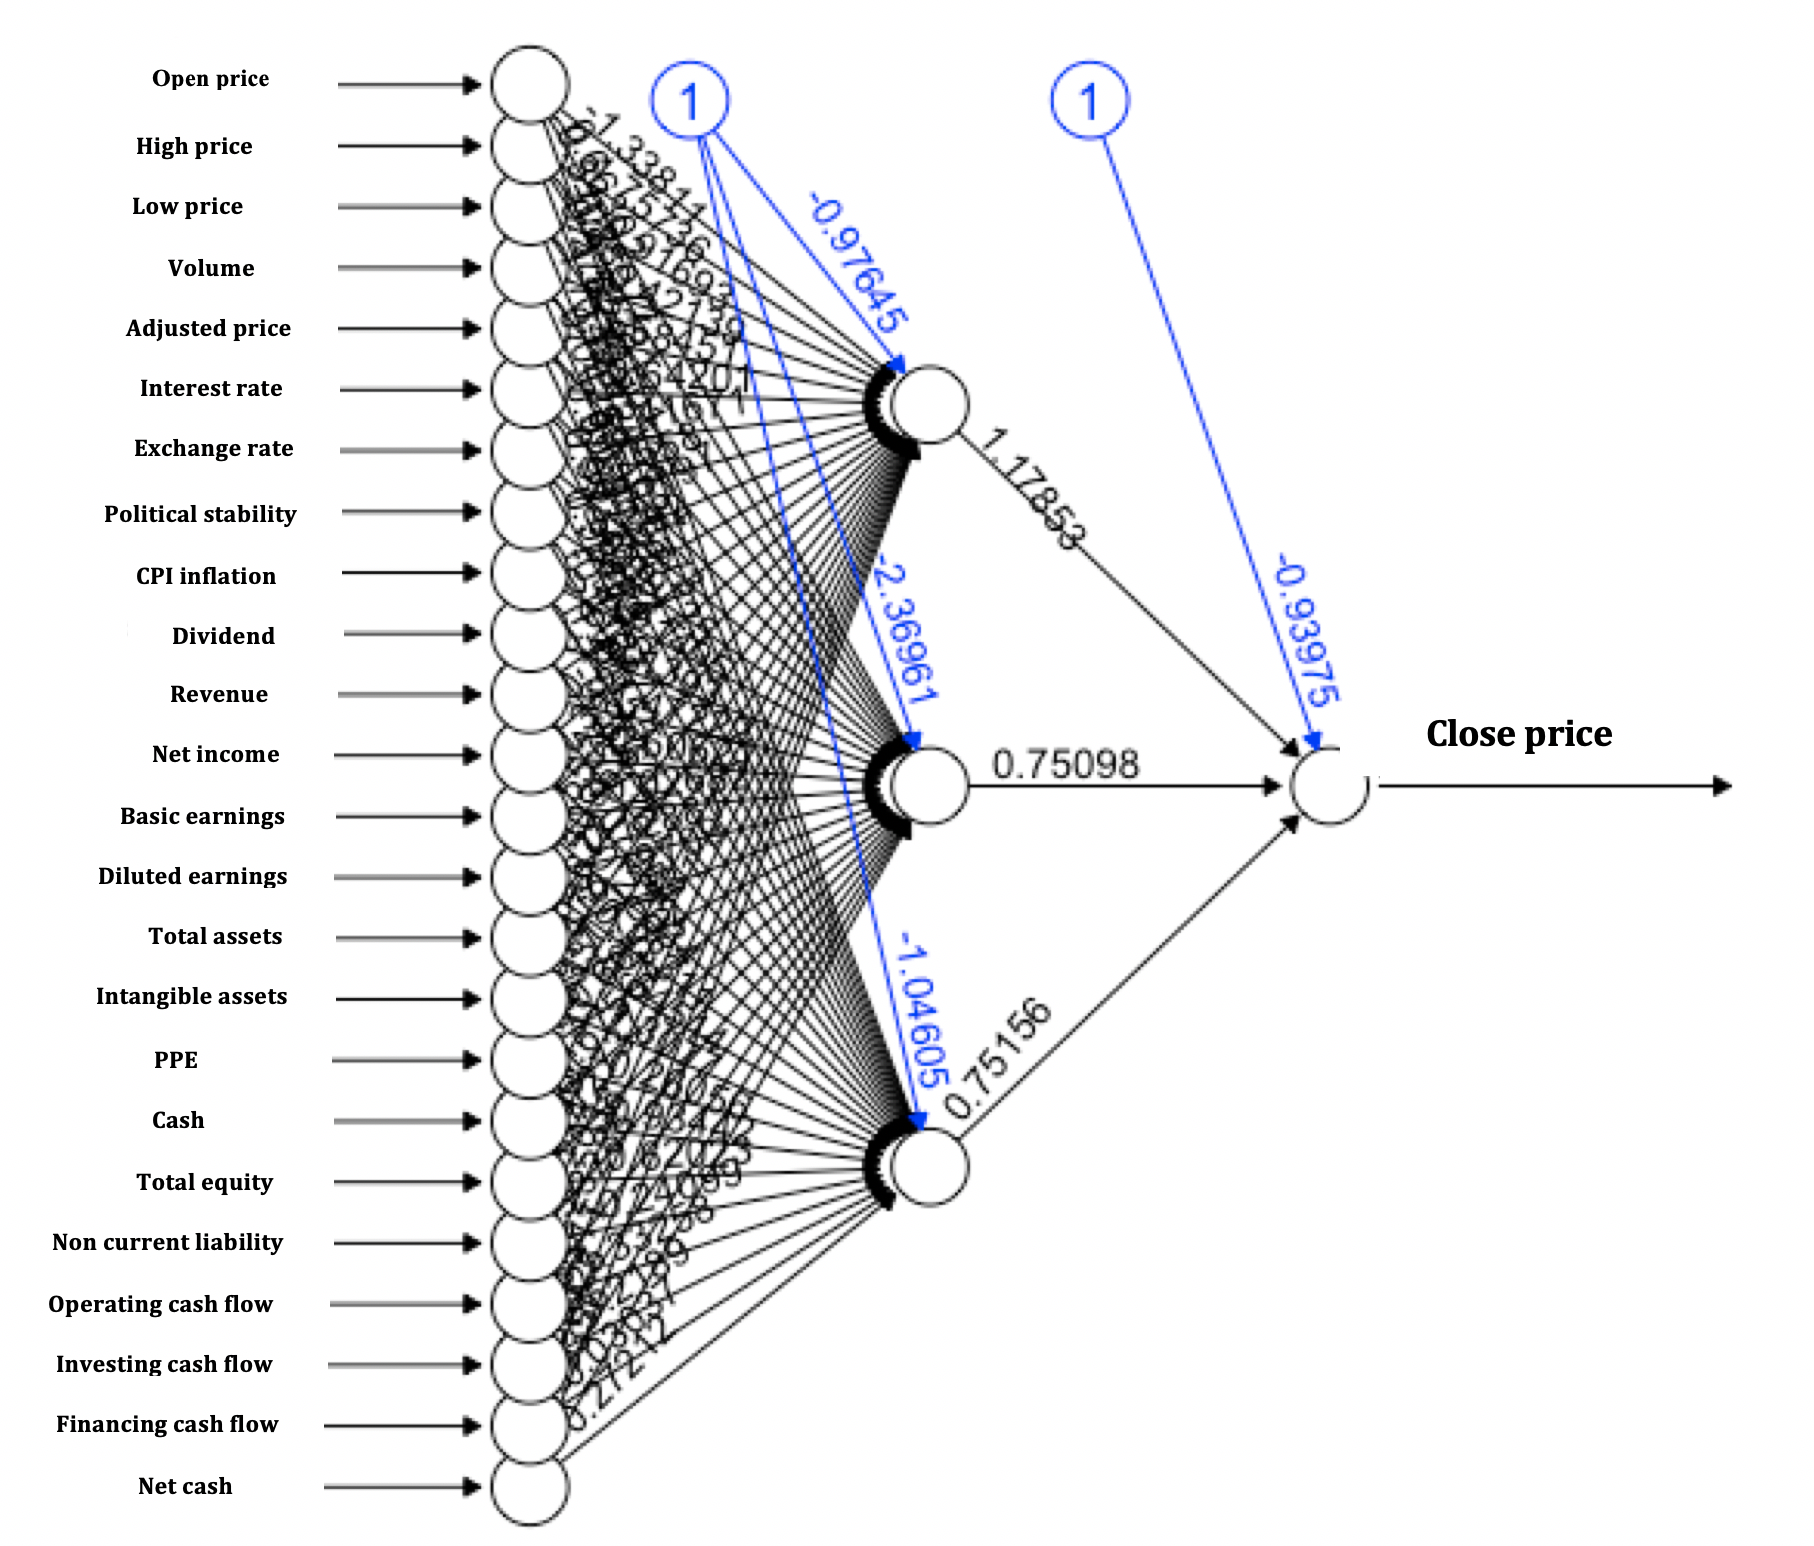
\includegraphics{D:/2017-2018/data_analysis/technical_analysis/report/NNrep.png}
\caption{Caption for the picture.}
\end{figure}

\begin{Shaded}
\begin{Highlighting}[]
\NormalTok{predict_testNN =}\StringTok{ }\KeywordTok{compute}\NormalTok{(NN, testNN[,}\KeywordTok{c}\NormalTok{(}\DecValTok{2}\OperatorTok{:}\DecValTok{25}\NormalTok{)])}
\CommentTok{# We descale the output to obtain the results in the real scale}
\NormalTok{predict_testNN =}\StringTok{ }\NormalTok{(predict_testNN}\OperatorTok{$}\NormalTok{net.result }\OperatorTok{*}\StringTok{ }\NormalTok{(}\KeywordTok{max}\NormalTok{(data}\OperatorTok{$}\NormalTok{A1) }\OperatorTok{-}\StringTok{ }\KeywordTok{min}\NormalTok{(data}\OperatorTok{$}\NormalTok{A1)))}
\OperatorTok{+}\StringTok{ }\KeywordTok{min}\NormalTok{(data}\OperatorTok{$}\NormalTok{A1)}
\CommentTok{# We create an array where to store the results per day for each stck}
\NormalTok{AI.P <-}\StringTok{ }\KeywordTok{c}\NormalTok{()}
\KeywordTok{View}\NormalTok{(data)}
\KeywordTok{View}\NormalTok{(data)}
\CommentTok{# We run the model for every single day per stock, to predict the prices }
\CommentTok{# one by one}
\KeywordTok{View}\NormalTok{(predict_testNN)}
\ControlFlowTok{for}\NormalTok{ (n }\ControlFlowTok{in} \DecValTok{1}\OperatorTok{:}\DecValTok{30}\NormalTok{)\{}
\NormalTok{  datatrain =}\StringTok{ }\NormalTok{data[ }\DecValTok{1}\OperatorTok{:}\DecValTok{1501}\OperatorTok{+}\NormalTok{n, ]}
\NormalTok{  datatest =}\StringTok{ }\NormalTok{data[ }\DecValTok{1502}\OperatorTok{+}\NormalTok{n, ]}
\NormalTok{  max =}\StringTok{ }\KeywordTok{apply}\NormalTok{(data , }\DecValTok{2}\NormalTok{ , max)}
\NormalTok{  min =}\StringTok{ }\KeywordTok{apply}\NormalTok{(data, }\DecValTok{2}\NormalTok{ , min)}
\NormalTok{  scaled =}\StringTok{ }\KeywordTok{as.data.frame}\NormalTok{(}\KeywordTok{scale}\NormalTok{(data, }\DataTypeTok{center =}\NormalTok{ min, }\DataTypeTok{scale =}\NormalTok{ max }\OperatorTok{-}\StringTok{ }\NormalTok{min))}
\NormalTok{  trainNN =}\StringTok{ }\NormalTok{scaled[}\DecValTok{1}\OperatorTok{:}\DecValTok{1501}\OperatorTok{+}\NormalTok{n , ]}
\NormalTok{  testNN =}\StringTok{ }\NormalTok{scaled[}\DecValTok{1502}\OperatorTok{+}\NormalTok{n , ]}
\CommentTok{# model with financial statements data}
\NormalTok{  NN =}\StringTok{ }\KeywordTok{neuralnet}\NormalTok{(A1 }\OperatorTok{~}\StringTok{ }\NormalTok{A2 }\OperatorTok{+}\StringTok{ }\NormalTok{A3 }\OperatorTok{+}\StringTok{ }\NormalTok{A4 }\OperatorTok{+}\StringTok{ }\NormalTok{A5 }\OperatorTok{+}\StringTok{ }\NormalTok{A6 }\OperatorTok{+}\StringTok{ }\NormalTok{A7 }\OperatorTok{+}\StringTok{ }\NormalTok{A8 }\OperatorTok{+}\StringTok{ }\NormalTok{A9 }\OperatorTok{+}\StringTok{ }\NormalTok{A10}
  \OperatorTok{+}\StringTok{ }\NormalTok{A11 }\OperatorTok{+}\StringTok{ }\NormalTok{A12 }\OperatorTok{+}\StringTok{ }\NormalTok{A13 }\OperatorTok{+}\StringTok{ }\NormalTok{A14 }\OperatorTok{+}\StringTok{ }\NormalTok{A15 }\OperatorTok{+}\StringTok{ }\NormalTok{A16 }\OperatorTok{+}\StringTok{ }\NormalTok{A17 }\OperatorTok{+}\StringTok{ }\NormalTok{A18 }\OperatorTok{+}\StringTok{ }\NormalTok{A19 }\OperatorTok{+}\StringTok{ }\NormalTok{A20 }\OperatorTok{+}\StringTok{ }\NormalTok{A21}
  \OperatorTok{+}\StringTok{ }\NormalTok{A22 }\OperatorTok{+}\StringTok{ }\NormalTok{A23 }\OperatorTok{+}\StringTok{ }\NormalTok{A24 }\OperatorTok{+}\StringTok{ }\NormalTok{A25, trainNN, }\DataTypeTok{hidden =} \DecValTok{3}\NormalTok{ , }\DataTypeTok{linear.output =}\NormalTok{ T )}
\NormalTok{  predict_testNN =}\StringTok{ }\KeywordTok{compute}\NormalTok{(NN, testNN[,}\KeywordTok{c}\NormalTok{(}\DecValTok{2}\OperatorTok{:}\DecValTok{25}\NormalTok{)])}
\NormalTok{  predict_testNN =}\StringTok{ }\NormalTok{(predict_testNN}\OperatorTok{$}\NormalTok{net.result }\OperatorTok{*}\StringTok{ }\NormalTok{(}\KeywordTok{max}\NormalTok{(data}\OperatorTok{$}\NormalTok{A1) }\OperatorTok{-}\StringTok{ }\KeywordTok{min}\NormalTok{(data}\OperatorTok{$}\NormalTok{A1)))}
  \OperatorTok{+}\StringTok{ }\KeywordTok{min}\NormalTok{(data}\OperatorTok{$}\NormalTok{A1)}
\NormalTok{  AI.P[n] <-}\StringTok{ }\NormalTok{predict_testNN}
\NormalTok{\}}
\KeywordTok{View}\NormalTok{(AI.P)}
\NormalTok{AI.P2 <-}\StringTok{ }\KeywordTok{c}\NormalTok{()}
\ControlFlowTok{for}\NormalTok{ (n }\ControlFlowTok{in} \DecValTok{1}\OperatorTok{:}\DecValTok{30}\NormalTok{)\{}
\NormalTok{  datatrain =}\StringTok{ }\NormalTok{data[ }\DecValTok{1}\OperatorTok{:}\DecValTok{1501}\OperatorTok{+}\NormalTok{n, ]}
\NormalTok{  datatest =}\StringTok{ }\NormalTok{data[ }\DecValTok{1502}\OperatorTok{+}\NormalTok{n, ]}
\NormalTok{  max =}\StringTok{ }\KeywordTok{apply}\NormalTok{(data , }\DecValTok{2}\NormalTok{ , max)}
\NormalTok{  min =}\StringTok{ }\KeywordTok{apply}\NormalTok{(data, }\DecValTok{2}\NormalTok{ , min)}
\NormalTok{  scaled =}\StringTok{ }\KeywordTok{as.data.frame}\NormalTok{(}\KeywordTok{scale}\NormalTok{(data, }\DataTypeTok{center =}\NormalTok{ min, }\DataTypeTok{scale =}\NormalTok{ max }\OperatorTok{-}\StringTok{ }\NormalTok{min))}
\NormalTok{  trainNN =}\StringTok{ }\NormalTok{scaled[}\DecValTok{1}\OperatorTok{:}\DecValTok{1501}\OperatorTok{+}\NormalTok{n , ]}
\NormalTok{  testNN =}\StringTok{ }\NormalTok{scaled[}\DecValTok{1502}\OperatorTok{+}\NormalTok{n , ]}
\CommentTok{# model without financial statements data}
\NormalTok{  NN =}\StringTok{ }\KeywordTok{neuralnet}\NormalTok{(A1 }\OperatorTok{~}\StringTok{ }\NormalTok{A2 }\OperatorTok{+}\StringTok{ }\NormalTok{A3 }\OperatorTok{+}\StringTok{ }\NormalTok{A4 }\OperatorTok{+}\StringTok{ }\NormalTok{A5 }\OperatorTok{+}\StringTok{ }\NormalTok{A6 }\OperatorTok{+}\StringTok{ }\NormalTok{A7 }\OperatorTok{+}\StringTok{ }\NormalTok{A8 }\OperatorTok{+}\StringTok{ }\NormalTok{A9 }\OperatorTok{+}\StringTok{ }\NormalTok{A10,}
\NormalTok{  trainNN, }\DataTypeTok{hidden =} \DecValTok{3}\NormalTok{ , }\DataTypeTok{linear.output =}\NormalTok{ T )}
\NormalTok{  predict_testNN =}\StringTok{ }\KeywordTok{compute}\NormalTok{(NN, testNN[,}\KeywordTok{c}\NormalTok{(}\DecValTok{2}\OperatorTok{:}\DecValTok{10}\NormalTok{)])}
\NormalTok{  predict_testNN =}\StringTok{ }\NormalTok{(predict_testNN}\OperatorTok{$}\NormalTok{net.result }\OperatorTok{*}\StringTok{ }\NormalTok{(}\KeywordTok{max}\NormalTok{(data}\OperatorTok{$}\NormalTok{A1) }\OperatorTok{-}\StringTok{ }\KeywordTok{min}\NormalTok{(data}\OperatorTok{$}\NormalTok{A1)))}
  \OperatorTok{+}\StringTok{ }\KeywordTok{min}\NormalTok{(data}\OperatorTok{$}\NormalTok{A1)}
\NormalTok{  AI.P2[n] <-}\StringTok{ }\NormalTok{predict_testNN}
\NormalTok{\}}
\CommentTok{# Calculate Root Mean Square Error (RMSE)}
\NormalTok{Reals <-}\StringTok{ }\NormalTok{data[}\DecValTok{1503}\OperatorTok{:}\DecValTok{1532}\NormalTok{,}\DecValTok{1}\NormalTok{]}
\KeywordTok{View}\NormalTok{(Reals)}
\KeywordTok{View}\NormalTok{(data)}
\NormalTok{RMSE <-}\StringTok{ }\KeywordTok{sqrt}\NormalTok{(}\KeywordTok{sum}\NormalTok{((Reals}\OperatorTok{-}\NormalTok{AI.P)}\OperatorTok{^}\DecValTok{2}\NormalTok{)) }\CommentTok{# RMSE = 6.072}
\NormalTok{RMSE2 <-}\StringTok{ }\KeywordTok{sqrt}\NormalTok{(}\KeywordTok{sum}\NormalTok{((Reals}\OperatorTok{-}\NormalTok{AI.P2)}\OperatorTok{^}\DecValTok{2}\NormalTok{)) }\CommentTok{# RMSE2 = 6.064}
\KeywordTok{View}\NormalTok{(AI.P)}
\end{Highlighting}
\end{Shaded}

As can be seen, the model without the financial statement variables
(RMSE = 6.072) is more accurate than the model with them (RMSE2 = 6.064)
according to the RMSE value. Hence, we will continue without taking into
account the financial statement variables.

\begin{Shaded}
\begin{Highlighting}[]
\CommentTok{#We predict the prices of the other 4 stocks one by one,}
\CommentTok{#without the financial statement variables as input}
\KeywordTok{library}\NormalTok{(readr)}
\NormalTok{AIR1 <-}\StringTok{ }\KeywordTok{read_csv2}\NormalTok{(}\StringTok{"D:/2017-2018/data_analysis/technical_analysis/data/AIR1.csv"}\NormalTok{)}
\NormalTok{data <-}\StringTok{ }\NormalTok{AIR1}
\NormalTok{AIR.P2 <-}\StringTok{ }\KeywordTok{c}\NormalTok{()}
\KeywordTok{View}\NormalTok{(data)}
\ControlFlowTok{for}\NormalTok{ (n }\ControlFlowTok{in} \DecValTok{1}\OperatorTok{:}\DecValTok{30}\NormalTok{)\{}
\NormalTok{  datatrain =}\StringTok{ }\NormalTok{data[ }\DecValTok{1}\OperatorTok{:}\DecValTok{1501}\OperatorTok{+}\NormalTok{n, ]}
\NormalTok{  datatest =}\StringTok{ }\NormalTok{data[ }\DecValTok{1502}\OperatorTok{+}\NormalTok{n, ]}
\NormalTok{  max =}\StringTok{ }\KeywordTok{apply}\NormalTok{(data , }\DecValTok{2}\NormalTok{ , max)}
\NormalTok{  min =}\StringTok{ }\KeywordTok{apply}\NormalTok{(data, }\DecValTok{2}\NormalTok{ , min)}
\NormalTok{  scaled =}\StringTok{ }\KeywordTok{as.data.frame}\NormalTok{(}\KeywordTok{scale}\NormalTok{(data, }\DataTypeTok{center =}\NormalTok{ min, }\DataTypeTok{scale =}\NormalTok{ max }\OperatorTok{-}\StringTok{ }\NormalTok{min))}
\NormalTok{  trainNN =}\StringTok{ }\NormalTok{scaled[}\DecValTok{1}\OperatorTok{:}\DecValTok{1501}\OperatorTok{+}\NormalTok{n , ]}
\NormalTok{  testNN =}\StringTok{ }\NormalTok{scaled[}\DecValTok{1502}\OperatorTok{+}\NormalTok{n , ]}
\NormalTok{  NN =}\StringTok{ }\KeywordTok{neuralnet}\NormalTok{(A1 }\OperatorTok{~}\StringTok{ }\NormalTok{A2 }\OperatorTok{+}\StringTok{ }\NormalTok{A3 }\OperatorTok{+}\StringTok{ }\NormalTok{A4 }\OperatorTok{+}\StringTok{ }\NormalTok{A5 }\OperatorTok{+}\StringTok{ }\NormalTok{A6 }\OperatorTok{+}\StringTok{ }\NormalTok{A7 }\OperatorTok{+}\StringTok{ }\NormalTok{A8 }\OperatorTok{+}\StringTok{ }\NormalTok{A9 }\OperatorTok{+}\StringTok{ }\NormalTok{A10,}
\NormalTok{  trainNN, }\DataTypeTok{hidden =} \DecValTok{3}\NormalTok{ , }\DataTypeTok{linear.output =}\NormalTok{ T )}
\NormalTok{  predict_testNN =}\StringTok{ }\KeywordTok{compute}\NormalTok{(NN, testNN[,}\KeywordTok{c}\NormalTok{(}\DecValTok{2}\OperatorTok{:}\DecValTok{10}\NormalTok{)])}
\NormalTok{  predict_testNN =}\StringTok{ }\NormalTok{(predict_testNN}\OperatorTok{$}\NormalTok{net.result }\OperatorTok{*}\StringTok{ }\NormalTok{(}\KeywordTok{max}\NormalTok{(data}\OperatorTok{$}\NormalTok{A1) }\OperatorTok{-}\StringTok{ }\KeywordTok{min}\NormalTok{(data}\OperatorTok{$}\NormalTok{A1)))}
  \OperatorTok{+}\StringTok{ }\KeywordTok{min}\NormalTok{(data}\OperatorTok{$}\NormalTok{A1)}
\NormalTok{  AIR.P2[n] <-}\StringTok{ }\NormalTok{predict_testNN}
\NormalTok{\}}
\NormalTok{BN.P2 <-}\StringTok{ }\KeywordTok{c}\NormalTok{()}
\KeywordTok{library}\NormalTok{(readr)}
\NormalTok{BN1 <-}\StringTok{ }\KeywordTok{read_csv2}\NormalTok{(}\StringTok{"D:/2017-2018/data_analysis/technical_analysis/data/BN1.csv"}\NormalTok{)}
\KeywordTok{View}\NormalTok{(BN1)}
\ControlFlowTok{for}\NormalTok{ (n }\ControlFlowTok{in} \DecValTok{1}\OperatorTok{:}\DecValTok{30}\NormalTok{)\{}
\NormalTok{  datatrain =}\StringTok{ }\NormalTok{data[ }\DecValTok{1}\OperatorTok{:}\DecValTok{1501}\OperatorTok{+}\NormalTok{n, ]}
\NormalTok{  datatest =}\StringTok{ }\NormalTok{data[ }\DecValTok{1502}\OperatorTok{+}\NormalTok{n, ]}
\NormalTok{  max =}\StringTok{ }\KeywordTok{apply}\NormalTok{(data , }\DecValTok{2}\NormalTok{ , max)}
\NormalTok{  min =}\StringTok{ }\KeywordTok{apply}\NormalTok{(data, }\DecValTok{2}\NormalTok{ , min)}
\NormalTok{  scaled =}\StringTok{ }\KeywordTok{as.data.frame}\NormalTok{(}\KeywordTok{scale}\NormalTok{(data, }\DataTypeTok{center =}\NormalTok{ min, }\DataTypeTok{scale =}\NormalTok{ max }\OperatorTok{-}\StringTok{ }\NormalTok{min))}
\NormalTok{  trainNN =}\StringTok{ }\NormalTok{scaled[}\DecValTok{1}\OperatorTok{:}\DecValTok{1501}\OperatorTok{+}\NormalTok{n , ]}
\NormalTok{  testNN =}\StringTok{ }\NormalTok{scaled[}\DecValTok{1502}\OperatorTok{+}\NormalTok{n , ]}
\NormalTok{  NN =}\StringTok{ }\KeywordTok{neuralnet}\NormalTok{(A1 }\OperatorTok{~}\StringTok{ }\NormalTok{A2 }\OperatorTok{+}\StringTok{ }\NormalTok{A3 }\OperatorTok{+}\StringTok{ }\NormalTok{A4 }\OperatorTok{+}\StringTok{ }\NormalTok{A5 }\OperatorTok{+}\StringTok{ }\NormalTok{A6 }\OperatorTok{+}\StringTok{ }\NormalTok{A7 }\OperatorTok{+}\StringTok{ }\NormalTok{A8 }\OperatorTok{+}\StringTok{ }\NormalTok{A9 }\OperatorTok{+}\StringTok{ }\NormalTok{A10,}
\NormalTok{  trainNN, }\DataTypeTok{hidden =} \DecValTok{3}\NormalTok{ , }\DataTypeTok{linear.output =}\NormalTok{ T )}
\NormalTok{  predict_testNN =}\StringTok{ }\KeywordTok{compute}\NormalTok{(NN, testNN[,}\KeywordTok{c}\NormalTok{(}\DecValTok{2}\OperatorTok{:}\DecValTok{10}\NormalTok{)])}
\NormalTok{  predict_testNN =}\StringTok{ }\NormalTok{(predict_testNN}\OperatorTok{$}\NormalTok{net.result }\OperatorTok{*}\StringTok{ }\NormalTok{(}\KeywordTok{max}\NormalTok{(data}\OperatorTok{$}\NormalTok{A1) }\OperatorTok{-}\StringTok{ }\KeywordTok{min}\NormalTok{(data}\OperatorTok{$}\NormalTok{A1)))}
  \OperatorTok{+}\StringTok{ }\KeywordTok{min}\NormalTok{(data}\OperatorTok{$}\NormalTok{A1)}
\NormalTok{  BN.P2[n] <-}\StringTok{ }\NormalTok{predict_testNN}
\NormalTok{\}}
\KeywordTok{View}\NormalTok{(data)}
\NormalTok{data <-}\StringTok{ }\NormalTok{BN1}
\KeywordTok{View}\NormalTok{(data)}
\ControlFlowTok{for}\NormalTok{ (n }\ControlFlowTok{in} \DecValTok{1}\OperatorTok{:}\DecValTok{30}\NormalTok{)\{}
\NormalTok{  datatrain =}\StringTok{ }\NormalTok{data[ }\DecValTok{1}\OperatorTok{:}\DecValTok{1501}\OperatorTok{+}\NormalTok{n, ]}
\NormalTok{  datatest =}\StringTok{ }\NormalTok{data[ }\DecValTok{1502}\OperatorTok{+}\NormalTok{n, ]}
\NormalTok{  max =}\StringTok{ }\KeywordTok{apply}\NormalTok{(data , }\DecValTok{2}\NormalTok{ , max)}
\NormalTok{  min =}\StringTok{ }\KeywordTok{apply}\NormalTok{(data, }\DecValTok{2}\NormalTok{ , min)}
\NormalTok{  scaled =}\StringTok{ }\KeywordTok{as.data.frame}\NormalTok{(}\KeywordTok{scale}\NormalTok{(data, }\DataTypeTok{center =}\NormalTok{ min, }\DataTypeTok{scale =}\NormalTok{ max }\OperatorTok{-}\StringTok{ }\NormalTok{min))}
\NormalTok{  trainNN =}\StringTok{ }\NormalTok{scaled[}\DecValTok{1}\OperatorTok{:}\DecValTok{1501}\OperatorTok{+}\NormalTok{n , ]}
\NormalTok{  testNN =}\StringTok{ }\NormalTok{scaled[}\DecValTok{1502}\OperatorTok{+}\NormalTok{n , ]}
\NormalTok{  NN =}\StringTok{ }\KeywordTok{neuralnet}\NormalTok{(A1 }\OperatorTok{~}\StringTok{ }\NormalTok{A2 }\OperatorTok{+}\StringTok{ }\NormalTok{A3 }\OperatorTok{+}\StringTok{ }\NormalTok{A4 }\OperatorTok{+}\StringTok{ }\NormalTok{A5 }\OperatorTok{+}\StringTok{ }\NormalTok{A6 }\OperatorTok{+}\StringTok{ }\NormalTok{A7 }\OperatorTok{+}\StringTok{ }\NormalTok{A8 }\OperatorTok{+}\StringTok{ }\NormalTok{A9 }\OperatorTok{+}\StringTok{ }\NormalTok{A10,}
\NormalTok{  trainNN, }\DataTypeTok{hidden =} \DecValTok{3}\NormalTok{ , }\DataTypeTok{linear.output =}\NormalTok{ T )}
\NormalTok{  predict_testNN =}\StringTok{ }\KeywordTok{compute}\NormalTok{(NN, testNN[,}\KeywordTok{c}\NormalTok{(}\DecValTok{2}\OperatorTok{:}\DecValTok{10}\NormalTok{)])}
\NormalTok{  predict_testNN =}\StringTok{ }\NormalTok{(predict_testNN}\OperatorTok{$}\NormalTok{net.result }\OperatorTok{*}\StringTok{ }\NormalTok{(}\KeywordTok{max}\NormalTok{(data}\OperatorTok{$}\NormalTok{A1) }\OperatorTok{-}\StringTok{ }\KeywordTok{min}\NormalTok{(data}\OperatorTok{$}\NormalTok{A1)))}
  \OperatorTok{+}\StringTok{ }\KeywordTok{min}\NormalTok{(data}\OperatorTok{$}\NormalTok{A1)}
\NormalTok{  BN.P2[n] <-}\StringTok{ }\NormalTok{predict_testNN}
\NormalTok{\}}
\KeywordTok{library}\NormalTok{(readr)}
\NormalTok{BNP1 <-}\StringTok{ }\KeywordTok{read_csv2}\NormalTok{(}\StringTok{"D:/2017-2018/data_analysis/technical_analysis/data/BNP1.csv"}\NormalTok{)}
\KeywordTok{View}\NormalTok{(BNP1)}
\NormalTok{data <-}\StringTok{ }\NormalTok{BNP1}
\KeywordTok{View}\NormalTok{(data)}
\NormalTok{BNP.P2 <-}\StringTok{ }\KeywordTok{c}\NormalTok{()}
\ControlFlowTok{for}\NormalTok{ (n }\ControlFlowTok{in} \DecValTok{1}\OperatorTok{:}\DecValTok{30}\NormalTok{)\{}
\NormalTok{  datatrain =}\StringTok{ }\NormalTok{data[ }\DecValTok{1}\OperatorTok{:}\DecValTok{1501}\OperatorTok{+}\NormalTok{n, ]}
\NormalTok{  datatest =}\StringTok{ }\NormalTok{data[ }\DecValTok{1502}\OperatorTok{+}\NormalTok{n, ]}
\NormalTok{  max =}\StringTok{ }\KeywordTok{apply}\NormalTok{(data , }\DecValTok{2}\NormalTok{ , max)}
\NormalTok{  min =}\StringTok{ }\KeywordTok{apply}\NormalTok{(data, }\DecValTok{2}\NormalTok{ , min)}
\NormalTok{  scaled =}\StringTok{ }\KeywordTok{as.data.frame}\NormalTok{(}\KeywordTok{scale}\NormalTok{(data, }\DataTypeTok{center =}\NormalTok{ min, }\DataTypeTok{scale =}\NormalTok{ max }\OperatorTok{-}\StringTok{ }\NormalTok{min))}
\NormalTok{  trainNN =}\StringTok{ }\NormalTok{scaled[}\DecValTok{1}\OperatorTok{:}\DecValTok{1501}\OperatorTok{+}\NormalTok{n , ]}
\NormalTok{  testNN =}\StringTok{ }\NormalTok{scaled[}\DecValTok{1502}\OperatorTok{+}\NormalTok{n , ]}
\NormalTok{  NN =}\StringTok{ }\KeywordTok{neuralnet}\NormalTok{(A1 }\OperatorTok{~}\StringTok{ }\NormalTok{A2 }\OperatorTok{+}\StringTok{ }\NormalTok{A3 }\OperatorTok{+}\StringTok{ }\NormalTok{A4 }\OperatorTok{+}\StringTok{ }\NormalTok{A5 }\OperatorTok{+}\StringTok{ }\NormalTok{A6 }\OperatorTok{+}\StringTok{ }\NormalTok{A7 }\OperatorTok{+}\StringTok{ }\NormalTok{A8 }\OperatorTok{+}\StringTok{ }\NormalTok{A9 }\OperatorTok{+}\StringTok{ }\NormalTok{A10,}
\NormalTok{  trainNN, }\DataTypeTok{hidden =} \DecValTok{3}\NormalTok{ , }\DataTypeTok{linear.output =}\NormalTok{ T )}
\NormalTok{  predict_testNN =}\StringTok{ }\KeywordTok{compute}\NormalTok{(NN, testNN[,}\KeywordTok{c}\NormalTok{(}\DecValTok{2}\OperatorTok{:}\DecValTok{10}\NormalTok{)])}
\NormalTok{  predict_testNN =}\StringTok{ }\NormalTok{(predict_testNN}\OperatorTok{$}\NormalTok{net.result }\OperatorTok{*}\StringTok{ }\NormalTok{(}\KeywordTok{max}\NormalTok{(data}\OperatorTok{$}\NormalTok{A1) }\OperatorTok{-}\StringTok{ }\KeywordTok{min}\NormalTok{(data}\OperatorTok{$}\NormalTok{A1)))}
  \OperatorTok{+}\StringTok{ }\KeywordTok{min}\NormalTok{(data}\OperatorTok{$}\NormalTok{A1)}
\NormalTok{  BNP.P2[n] <-}\StringTok{ }\NormalTok{predict_testNN}
\NormalTok{\}}
\NormalTok{DG.P2 <-}\StringTok{ }\KeywordTok{c}\NormalTok{()}
\KeywordTok{library}\NormalTok{(readr)}
\NormalTok{DG1 <-}\StringTok{ }\KeywordTok{read_csv2}\NormalTok{(}\StringTok{"D:/2017-2018/data_analysis/technical_analysis/data/DG1.csv"}\NormalTok{)}
\KeywordTok{View}\NormalTok{(DG1)}
\NormalTok{data <-}\StringTok{ }\NormalTok{DG1}
\KeywordTok{View}\NormalTok{(data)}
\ControlFlowTok{for}\NormalTok{ (n }\ControlFlowTok{in} \DecValTok{1}\OperatorTok{:}\DecValTok{30}\NormalTok{)\{}
\NormalTok{  datatrain =}\StringTok{ }\NormalTok{data[ }\DecValTok{1}\OperatorTok{:}\DecValTok{1501}\OperatorTok{+}\NormalTok{n, ]}
\NormalTok{  datatest =}\StringTok{ }\NormalTok{data[ }\DecValTok{1502}\OperatorTok{+}\NormalTok{n, ]}
\NormalTok{  max =}\StringTok{ }\KeywordTok{apply}\NormalTok{(data , }\DecValTok{2}\NormalTok{ , max)}
\NormalTok{  min =}\StringTok{ }\KeywordTok{apply}\NormalTok{(data, }\DecValTok{2}\NormalTok{ , min)}
\NormalTok{  scaled =}\StringTok{ }\KeywordTok{as.data.frame}\NormalTok{(}\KeywordTok{scale}\NormalTok{(data, }\DataTypeTok{center =}\NormalTok{ min, }\DataTypeTok{scale =}\NormalTok{ max }\OperatorTok{-}\StringTok{ }\NormalTok{min))}
\NormalTok{  trainNN =}\StringTok{ }\NormalTok{scaled[}\DecValTok{1}\OperatorTok{:}\DecValTok{1501}\OperatorTok{+}\NormalTok{n , ]}
\NormalTok{  testNN =}\StringTok{ }\NormalTok{scaled[}\DecValTok{1502}\OperatorTok{+}\NormalTok{n , ]}
\NormalTok{  NN =}\StringTok{ }\KeywordTok{neuralnet}\NormalTok{(A1 }\OperatorTok{~}\StringTok{ }\NormalTok{A2 }\OperatorTok{+}\StringTok{ }\NormalTok{A3 }\OperatorTok{+}\StringTok{ }\NormalTok{A4 }\OperatorTok{+}\StringTok{ }\NormalTok{A5 }\OperatorTok{+}\StringTok{ }\NormalTok{A6 }\OperatorTok{+}\StringTok{ }\NormalTok{A7 }\OperatorTok{+}\StringTok{ }\NormalTok{A8 }\OperatorTok{+}\StringTok{ }\NormalTok{A9 }\OperatorTok{+}\StringTok{ }\NormalTok{A10, }
\NormalTok{                 trainNN, }\DataTypeTok{hidden =} \DecValTok{3}\NormalTok{ , }\DataTypeTok{linear.output =}\NormalTok{ T )}
\NormalTok{  predict_testNN =}\StringTok{ }\KeywordTok{compute}\NormalTok{(NN, testNN[,}\KeywordTok{c}\NormalTok{(}\DecValTok{2}\OperatorTok{:}\DecValTok{10}\NormalTok{)])}
\NormalTok{  predict_testNN =}\StringTok{ }\NormalTok{(predict_testNN}\OperatorTok{$}\NormalTok{net.result }\OperatorTok{*}\StringTok{ }
\StringTok{                      }\NormalTok{(}\KeywordTok{max}\NormalTok{(data}\OperatorTok{$}\NormalTok{A1) }\OperatorTok{-}\StringTok{ }\KeywordTok{min}\NormalTok{(data}\OperatorTok{$}\NormalTok{A1))) }\OperatorTok{+}\StringTok{ }\KeywordTok{min}\NormalTok{(data}\OperatorTok{$}\NormalTok{A1)}
\NormalTok{  DG.P2[n] <-}\StringTok{ }\NormalTok{predict_testNN}
\NormalTok{\}}
\end{Highlighting}
\end{Shaded}

We want to create a table with the predicted daily increase in price for
every stock during the 30 days. After that, we will identify the stock
with the highest predicted increase in price for every day. This will be
the stock where to invest all the capital for the day.

\begin{Shaded}
\begin{Highlighting}[]
\KeywordTok{View}\NormalTok{(AIR.P2)}
\KeywordTok{View}\NormalTok{(AI1)}
\NormalTok{AI.R <-}\StringTok{ }\NormalTok{AI1[}\DecValTok{1502}\OperatorTok{:}\DecValTok{1531}\NormalTok{, }\KeywordTok{c}\NormalTok{(}\DecValTok{2}\NormalTok{)]}
\KeywordTok{View}\NormalTok{(AI.R)}
\KeywordTok{View}\NormalTok{(AI1)}
\KeywordTok{View}\NormalTok{(AIR1)}
\NormalTok{AIR.R <-}\StringTok{ }\NormalTok{AIR1[}\DecValTok{1502}\OperatorTok{:}\DecValTok{1531}\NormalTok{, }\KeywordTok{c}\NormalTok{(}\DecValTok{1}\NormalTok{)]}
\KeywordTok{View}\NormalTok{(BN1)}
\NormalTok{BN.R <-}\StringTok{ }\NormalTok{BN1[}\DecValTok{1502}\OperatorTok{:}\DecValTok{1531}\NormalTok{, }\KeywordTok{c}\NormalTok{(}\DecValTok{1}\NormalTok{)]}
\KeywordTok{View}\NormalTok{(BNP1)}
\NormalTok{BNP.R <-}\StringTok{ }\NormalTok{BNP1[}\DecValTok{1502}\OperatorTok{:}\DecValTok{1531}\NormalTok{, }\KeywordTok{c}\NormalTok{(}\DecValTok{1}\NormalTok{)]}
\KeywordTok{View}\NormalTok{(DG1)}
\NormalTok{DG.R <-}\StringTok{ }\NormalTok{DG1[}\DecValTok{1502}\OperatorTok{:}\DecValTok{1531}\NormalTok{, }\KeywordTok{c}\NormalTok{(}\DecValTok{1}\NormalTok{)]}
\NormalTok{AI.DIF <-}\StringTok{ }\NormalTok{AI.P2 }\OperatorTok{-}\StringTok{ }\NormalTok{AI.R}
\NormalTok{AIR.DIF <-}\StringTok{ }\NormalTok{AIR.P2 }\OperatorTok{-}\StringTok{ }\NormalTok{AIR.R}
\NormalTok{BN.DIF <-}\StringTok{ }\NormalTok{BN.P2 }\OperatorTok{-}\StringTok{ }\NormalTok{BN.R}
\NormalTok{BNP.DIF <-}\StringTok{ }\NormalTok{BNP.P2 }\OperatorTok{-}\StringTok{ }\NormalTok{BNP.R}
\NormalTok{DG.DIF <-}\StringTok{ }\NormalTok{DG.P2 }\OperatorTok{-}\StringTok{ }\NormalTok{DG.R}
\NormalTok{df =}\StringTok{ }\KeywordTok{data.frame}\NormalTok{(AI.DIF,AIR.DIF,BN.DIF,BNP.DIF,DG.DIF)}
\KeywordTok{View}\NormalTok{(df)}
\CommentTok{#identify the stock with the highest predicted increase in price for every day}
\NormalTok{X <-}\StringTok{ }\KeywordTok{c}\NormalTok{()}
\ControlFlowTok{for}\NormalTok{ (n }\ControlFlowTok{in} \DecValTok{1}\OperatorTok{:}\DecValTok{30}\NormalTok{)\{}
  \ControlFlowTok{if}\NormalTok{ (}\KeywordTok{max}\NormalTok{(df[n,]) }\OperatorTok{==}\StringTok{ }\NormalTok{df[n,}\StringTok{"A1"}\NormalTok{])\{}
\NormalTok{    X[n] =}\StringTok{ "AI.PA"}
\NormalTok{  \} }\ControlFlowTok{else} \ControlFlowTok{if}\NormalTok{ (}\KeywordTok{max}\NormalTok{(df[n,]) }\OperatorTok{==}\StringTok{ }\NormalTok{df[n,}\StringTok{"A1.1"}\NormalTok{])\{}
\NormalTok{    X[n] =}\StringTok{ "AIR.PA"}
\NormalTok{  \} }\ControlFlowTok{else} \ControlFlowTok{if}\NormalTok{ (}\KeywordTok{max}\NormalTok{(df[n,]) }\OperatorTok{==}\StringTok{ }\NormalTok{df[n,}\StringTok{"A1.2"}\NormalTok{])\{}
\NormalTok{    X[n] =}\StringTok{ "BN.PA"}
\NormalTok{  \} }\ControlFlowTok{else} \ControlFlowTok{if}\NormalTok{ (}\KeywordTok{max}\NormalTok{(df[n,]) }\OperatorTok{==}\StringTok{ }\NormalTok{df[n,}\StringTok{"A1.3"}\NormalTok{])\{}
\NormalTok{    X[n] =}\StringTok{ "BNP.PA"}
\NormalTok{  \} }\ControlFlowTok{else} \ControlFlowTok{if}\NormalTok{ (}\KeywordTok{max}\NormalTok{(df[n,]) }\OperatorTok{==}\StringTok{ }\NormalTok{df[n,}\StringTok{"A1.4"}\NormalTok{])\{}
\NormalTok{    X[n] =}\StringTok{ "DG.PA"}
\NormalTok{  \}}
\NormalTok{\}}
\KeywordTok{View}\NormalTok{(X)}
\end{Highlighting}
\end{Shaded}

\begin{longtable}[]{@{}llllllllll@{}}
\caption{Multiple-input NN strategy outcome}\tabularnewline
\toprule
\begin{minipage}[b]{0.04\columnwidth}\raggedright
Day\strut
\end{minipage} & \begin{minipage}[b]{0.09\columnwidth}\raggedright
Invest in\strut
\end{minipage} & \begin{minipage}[b]{0.10\columnwidth}\raggedright
date\strut
\end{minipage} & \begin{minipage}[b]{0.06\columnwidth}\raggedright
AI\strut
\end{minipage} & \begin{minipage}[b]{0.06\columnwidth}\raggedright
AIR\strut
\end{minipage} & \begin{minipage}[b]{0.06\columnwidth}\raggedright
BNP\strut
\end{minipage} & \begin{minipage}[b]{0.06\columnwidth}\raggedright
BN\strut
\end{minipage} & \begin{minipage}[b]{0.06\columnwidth}\raggedright
DG\strut
\end{minipage} & \begin{minipage}[b]{0.13\columnwidth}\raggedright
\#shares bought\strut
\end{minipage} & \begin{minipage}[b]{0.08\columnwidth}\raggedright
€ Value\strut
\end{minipage}\tabularnewline
\midrule
\endfirsthead
\toprule
\begin{minipage}[b]{0.04\columnwidth}\raggedright
Day\strut
\end{minipage} & \begin{minipage}[b]{0.09\columnwidth}\raggedright
Invest in\strut
\end{minipage} & \begin{minipage}[b]{0.10\columnwidth}\raggedright
date\strut
\end{minipage} & \begin{minipage}[b]{0.06\columnwidth}\raggedright
AI\strut
\end{minipage} & \begin{minipage}[b]{0.06\columnwidth}\raggedright
AIR\strut
\end{minipage} & \begin{minipage}[b]{0.06\columnwidth}\raggedright
BNP\strut
\end{minipage} & \begin{minipage}[b]{0.06\columnwidth}\raggedright
BN\strut
\end{minipage} & \begin{minipage}[b]{0.06\columnwidth}\raggedright
DG\strut
\end{minipage} & \begin{minipage}[b]{0.13\columnwidth}\raggedright
\#shares bought\strut
\end{minipage} & \begin{minipage}[b]{0.08\columnwidth}\raggedright
€ Value\strut
\end{minipage}\tabularnewline
\midrule
\endhead
\begin{minipage}[t]{0.04\columnwidth}\raggedright
1\strut
\end{minipage} & \begin{minipage}[t]{0.09\columnwidth}\raggedright
DG\strut
\end{minipage} & \begin{minipage}[t]{0.10\columnwidth}\raggedright
16/11/2018\strut
\end{minipage} & \begin{minipage}[t]{0.06\columnwidth}\raggedright
95.86\strut
\end{minipage} & \begin{minipage}[t]{0.06\columnwidth}\raggedright
92.88\strut
\end{minipage} & \begin{minipage}[t]{0.06\columnwidth}\raggedright
65.09\strut
\end{minipage} & \begin{minipage}[t]{0.06\columnwidth}\raggedright
45.19\strut
\end{minipage} & \begin{minipage}[t]{0.06\columnwidth}\raggedright
77.09\strut
\end{minipage} & \begin{minipage}[t]{0.13\columnwidth}\raggedright
129.70\strut
\end{minipage} & \begin{minipage}[t]{0.08\columnwidth}\raggedright
10000\strut
\end{minipage}\tabularnewline
\begin{minipage}[t]{0.04\columnwidth}\raggedright
2\strut
\end{minipage} & \begin{minipage}[t]{0.09\columnwidth}\raggedright
DG\strut
\end{minipage} & \begin{minipage}[t]{0.10\columnwidth}\raggedright
19/11/2018\strut
\end{minipage} & \begin{minipage}[t]{0.06\columnwidth}\raggedright
95.40\strut
\end{minipage} & \begin{minipage}[t]{0.06\columnwidth}\raggedright
92.57\strut
\end{minipage} & \begin{minipage}[t]{0.06\columnwidth}\raggedright
64.70\strut
\end{minipage} & \begin{minipage}[t]{0.06\columnwidth}\raggedright
45.28\strut
\end{minipage} & \begin{minipage}[t]{0.06\columnwidth}\raggedright
76.80\strut
\end{minipage} & \begin{minipage}[t]{0.13\columnwidth}\raggedright
129.70\strut
\end{minipage} & \begin{minipage}[t]{0.08\columnwidth}\raggedright
9961.09\strut
\end{minipage}\tabularnewline
\begin{minipage}[t]{0.04\columnwidth}\raggedright
3\strut
\end{minipage} & \begin{minipage}[t]{0.09\columnwidth}\raggedright
DG\strut
\end{minipage} & \begin{minipage}[t]{0.10\columnwidth}\raggedright
20/11/2018\strut
\end{minipage} & \begin{minipage}[t]{0.06\columnwidth}\raggedright
93.5\strut
\end{minipage} & \begin{minipage}[t]{0.06\columnwidth}\raggedright
91.07\strut
\end{minipage} & \begin{minipage}[t]{0.06\columnwidth}\raggedright
64.98\strut
\end{minipage} & \begin{minipage}[t]{0.06\columnwidth}\raggedright
44.30\strut
\end{minipage} & \begin{minipage}[t]{0.06\columnwidth}\raggedright
76.37\strut
\end{minipage} & \begin{minipage}[t]{0.13\columnwidth}\raggedright
129.70\strut
\end{minipage} & \begin{minipage}[t]{0.08\columnwidth}\raggedright
9906.61\strut
\end{minipage}\tabularnewline
\begin{minipage}[t]{0.04\columnwidth}\raggedright
4\strut
\end{minipage} & \begin{minipage}[t]{0.09\columnwidth}\raggedright
AIR\strut
\end{minipage} & \begin{minipage}[t]{0.10\columnwidth}\raggedright
21/11/2018\strut
\end{minipage} & \begin{minipage}[t]{0.06\columnwidth}\raggedright
94.22\strut
\end{minipage} & \begin{minipage}[t]{0.06\columnwidth}\raggedright
93.16\strut
\end{minipage} & \begin{minipage}[t]{0.06\columnwidth}\raggedright
65.41\strut
\end{minipage} & \begin{minipage}[t]{0.06\columnwidth}\raggedright
44.79\strut
\end{minipage} & \begin{minipage}[t]{0.06\columnwidth}\raggedright
77.01\strut
\end{minipage} & \begin{minipage}[t]{0.13\columnwidth}\raggedright
107.21\strut
\end{minipage} & \begin{minipage}[t]{0.08\columnwidth}\raggedright
9989.62\strut
\end{minipage}\tabularnewline
\begin{minipage}[t]{0.04\columnwidth}\raggedright
5\strut
\end{minipage} & \begin{minipage}[t]{0.09\columnwidth}\raggedright
AIR\strut
\end{minipage} & \begin{minipage}[t]{0.10\columnwidth}\raggedright
22/11/2018\strut
\end{minipage} & \begin{minipage}[t]{0.06\columnwidth}\raggedright
93.31\strut
\end{minipage} & \begin{minipage}[t]{0.06\columnwidth}\raggedright
92.33\strut
\end{minipage} & \begin{minipage}[t]{0.06\columnwidth}\raggedright
65.27\strut
\end{minipage} & \begin{minipage}[t]{0.06\columnwidth}\raggedright
44.28\strut
\end{minipage} & \begin{minipage}[t]{0.06\columnwidth}\raggedright
76.62\strut
\end{minipage} & \begin{minipage}[t]{0.13\columnwidth}\raggedright
107.21\strut
\end{minipage} & \begin{minipage}[t]{0.08\columnwidth}\raggedright
9899.55\strut
\end{minipage}\tabularnewline
\begin{minipage}[t]{0.04\columnwidth}\raggedright
6\strut
\end{minipage} & \begin{minipage}[t]{0.09\columnwidth}\raggedright
DG\strut
\end{minipage} & \begin{minipage}[t]{0.10\columnwidth}\raggedright
23/11/2018\strut
\end{minipage} & \begin{minipage}[t]{0.06\columnwidth}\raggedright
93.86\strut
\end{minipage} & \begin{minipage}[t]{0.06\columnwidth}\raggedright
93.41\strut
\end{minipage} & \begin{minipage}[t]{0.06\columnwidth}\raggedright
65.87\strut
\end{minipage} & \begin{minipage}[t]{0.06\columnwidth}\raggedright
44.36\strut
\end{minipage} & \begin{minipage}[t]{0.06\columnwidth}\raggedright
76.86\strut
\end{minipage} & \begin{minipage}[t]{0.13\columnwidth}\raggedright
130.30\strut
\end{minipage} & \begin{minipage}[t]{0.08\columnwidth}\raggedright
10015.35\strut
\end{minipage}\tabularnewline
\begin{minipage}[t]{0.04\columnwidth}\raggedright
7\strut
\end{minipage} & \begin{minipage}[t]{0.09\columnwidth}\raggedright
DG\strut
\end{minipage} & \begin{minipage}[t]{0.10\columnwidth}\raggedright
26/11/2018\strut
\end{minipage} & \begin{minipage}[t]{0.06\columnwidth}\raggedright
95.86\strut
\end{minipage} & \begin{minipage}[t]{0.06\columnwidth}\raggedright
93.58\strut
\end{minipage} & \begin{minipage}[t]{0.06\columnwidth}\raggedright
65.82\strut
\end{minipage} & \begin{minipage}[t]{0.06\columnwidth}\raggedright
45.34\strut
\end{minipage} & \begin{minipage}[t]{0.06\columnwidth}\raggedright
78.54\strut
\end{minipage} & \begin{minipage}[t]{0.13\columnwidth}\raggedright
130.30\strut
\end{minipage} & \begin{minipage}[t]{0.08\columnwidth}\raggedright
10234.27\strut
\end{minipage}\tabularnewline
\begin{minipage}[t]{0.04\columnwidth}\raggedright
8\strut
\end{minipage} & \begin{minipage}[t]{0.09\columnwidth}\raggedright
AIR\strut
\end{minipage} & \begin{minipage}[t]{0.10\columnwidth}\raggedright
27/11/2018\strut
\end{minipage} & \begin{minipage}[t]{0.06\columnwidth}\raggedright
94.86\strut
\end{minipage} & \begin{minipage}[t]{0.06\columnwidth}\raggedright
93.69\strut
\end{minipage} & \begin{minipage}[t]{0.06\columnwidth}\raggedright
66.41\strut
\end{minipage} & \begin{minipage}[t]{0.06\columnwidth}\raggedright
45.08\strut
\end{minipage} & \begin{minipage}[t]{0.06\columnwidth}\raggedright
78.16\strut
\end{minipage} & \begin{minipage}[t]{0.13\columnwidth}\raggedright
108.69\strut
\end{minipage} & \begin{minipage}[t]{0.08\columnwidth}\raggedright
10184.75\strut
\end{minipage}\tabularnewline
\begin{minipage}[t]{0.04\columnwidth}\raggedright
9\strut
\end{minipage} & \begin{minipage}[t]{0.09\columnwidth}\raggedright
DG\strut
\end{minipage} & \begin{minipage}[t]{0.10\columnwidth}\raggedright
28/11/2018\strut
\end{minipage} & \begin{minipage}[t]{0.06\columnwidth}\raggedright
94.36\strut
\end{minipage} & \begin{minipage}[t]{0.06\columnwidth}\raggedright
93.5\strut
\end{minipage} & \begin{minipage}[t]{0.06\columnwidth}\raggedright
65.41\strut
\end{minipage} & \begin{minipage}[t]{0.06\columnwidth}\raggedright
44.75\strut
\end{minipage} & \begin{minipage}[t]{0.06\columnwidth}\raggedright
77.95\strut
\end{minipage} & \begin{minipage}[t]{0.13\columnwidth}\raggedright
130.36\strut
\end{minipage} & \begin{minipage}[t]{0.08\columnwidth}\raggedright
10163.01\strut
\end{minipage}\tabularnewline
\begin{minipage}[t]{0.04\columnwidth}\raggedright
10\strut
\end{minipage} & \begin{minipage}[t]{0.09\columnwidth}\raggedright
DG\strut
\end{minipage} & \begin{minipage}[t]{0.10\columnwidth}\raggedright
29/11/2018\strut
\end{minipage} & \begin{minipage}[t]{0.06\columnwidth}\raggedright
94.68\strut
\end{minipage} & \begin{minipage}[t]{0.06\columnwidth}\raggedright
94.86\strut
\end{minipage} & \begin{minipage}[t]{0.06\columnwidth}\raggedright
65.54\strut
\end{minipage} & \begin{minipage}[t]{0.06\columnwidth}\raggedright
44.77\strut
\end{minipage} & \begin{minipage}[t]{0.06\columnwidth}\raggedright
77.58\strut
\end{minipage} & \begin{minipage}[t]{0.13\columnwidth}\raggedright
130.36\strut
\end{minipage} & \begin{minipage}[t]{0.08\columnwidth}\raggedright
10113.47\strut
\end{minipage}\tabularnewline
\begin{minipage}[t]{0.04\columnwidth}\raggedright
11\strut
\end{minipage} & \begin{minipage}[t]{0.09\columnwidth}\raggedright
DG\strut
\end{minipage} & \begin{minipage}[t]{0.10\columnwidth}\raggedright
30/11/2018\strut
\end{minipage} & \begin{minipage}[t]{0.06\columnwidth}\raggedright
97.04\strut
\end{minipage} & \begin{minipage}[t]{0.06\columnwidth}\raggedright
94.62\strut
\end{minipage} & \begin{minipage}[t]{0.06\columnwidth}\raggedright
66.05\strut
\end{minipage} & \begin{minipage}[t]{0.06\columnwidth}\raggedright
44.37\strut
\end{minipage} & \begin{minipage}[t]{0.06\columnwidth}\raggedright
77.09\strut
\end{minipage} & \begin{minipage}[t]{0.13\columnwidth}\raggedright
130.36\strut
\end{minipage} & \begin{minipage}[t]{0.08\columnwidth}\raggedright
10050.90\strut
\end{minipage}\tabularnewline
\begin{minipage}[t]{0.04\columnwidth}\raggedright
12\strut
\end{minipage} & \begin{minipage}[t]{0.09\columnwidth}\raggedright
DG\strut
\end{minipage} & \begin{minipage}[t]{0.10\columnwidth}\raggedright
03/12/2018\strut
\end{minipage} & \begin{minipage}[t]{0.06\columnwidth}\raggedright
97.27\strut
\end{minipage} & \begin{minipage}[t]{0.06\columnwidth}\raggedright
95.69\strut
\end{minipage} & \begin{minipage}[t]{0.06\columnwidth}\raggedright
65.41\strut
\end{minipage} & \begin{minipage}[t]{0.06\columnwidth}\raggedright
44.84\strut
\end{minipage} & \begin{minipage}[t]{0.06\columnwidth}\raggedright
75.40\strut
\end{minipage} & \begin{minipage}[t]{0.13\columnwidth}\raggedright
130.36\strut
\end{minipage} & \begin{minipage}[t]{0.08\columnwidth}\raggedright
9829.29\strut
\end{minipage}\tabularnewline
\begin{minipage}[t]{0.04\columnwidth}\raggedright
13\strut
\end{minipage} & \begin{minipage}[t]{0.09\columnwidth}\raggedright
DG\strut
\end{minipage} & \begin{minipage}[t]{0.10\columnwidth}\raggedright
04/12/2018\strut
\end{minipage} & \begin{minipage}[t]{0.06\columnwidth}\raggedright
97.45\strut
\end{minipage} & \begin{minipage}[t]{0.06\columnwidth}\raggedright
94.26\strut
\end{minipage} & \begin{minipage}[t]{0.06\columnwidth}\raggedright
65.52\strut
\end{minipage} & \begin{minipage}[t]{0.06\columnwidth}\raggedright
43.86\strut
\end{minipage} & \begin{minipage}[t]{0.06\columnwidth}\raggedright
76.66\strut
\end{minipage} & \begin{minipage}[t]{0.13\columnwidth}\raggedright
130.36\strut
\end{minipage} & \begin{minipage}[t]{0.08\columnwidth}\raggedright
9993.54\strut
\end{minipage}\tabularnewline
\begin{minipage}[t]{0.04\columnwidth}\raggedright
14\strut
\end{minipage} & \begin{minipage}[t]{0.09\columnwidth}\raggedright
AIR\strut
\end{minipage} & \begin{minipage}[t]{0.10\columnwidth}\raggedright
05/12/2018\strut
\end{minipage} & \begin{minipage}[t]{0.06\columnwidth}\raggedright
96.45\strut
\end{minipage} & \begin{minipage}[t]{0.06\columnwidth}\raggedright
92.30\strut
\end{minipage} & \begin{minipage}[t]{0.06\columnwidth}\raggedright
64.58\strut
\end{minipage} & \begin{minipage}[t]{0.06\columnwidth}\raggedright
43.41\strut
\end{minipage} & \begin{minipage}[t]{0.06\columnwidth}\raggedright
74.66\strut
\end{minipage} & \begin{minipage}[t]{0.13\columnwidth}\raggedright
105.43\strut
\end{minipage} & \begin{minipage}[t]{0.08\columnwidth}\raggedright
9732.82\strut
\end{minipage}\tabularnewline
\begin{minipage}[t]{0.04\columnwidth}\raggedright
15\strut
\end{minipage} & \begin{minipage}[t]{0.09\columnwidth}\raggedright
DG\strut
\end{minipage} & \begin{minipage}[t]{0.10\columnwidth}\raggedright
06/12/2018\strut
\end{minipage} & \begin{minipage}[t]{0.06\columnwidth}\raggedright
94.63\strut
\end{minipage} & \begin{minipage}[t]{0.06\columnwidth}\raggedright
88.63\strut
\end{minipage} & \begin{minipage}[t]{0.06\columnwidth}\raggedright
63.43\strut
\end{minipage} & \begin{minipage}[t]{0.06\columnwidth}\raggedright
41.78\strut
\end{minipage} & \begin{minipage}[t]{0.06\columnwidth}\raggedright
70.98\strut
\end{minipage} & \begin{minipage}[t]{0.13\columnwidth}\raggedright
131.66\strut
\end{minipage} & \begin{minipage}[t]{0.08\columnwidth}\raggedright
9345.87\strut
\end{minipage}\tabularnewline
\begin{minipage}[t]{0.04\columnwidth}\raggedright
16\strut
\end{minipage} & \begin{minipage}[t]{0.09\columnwidth}\raggedright
DG\strut
\end{minipage} & \begin{minipage}[t]{0.10\columnwidth}\raggedright
07/12/2018\strut
\end{minipage} & \begin{minipage}[t]{0.06\columnwidth}\raggedright
95.86\strut
\end{minipage} & \begin{minipage}[t]{0.06\columnwidth}\raggedright
89.07\strut
\end{minipage} & \begin{minipage}[t]{0.06\columnwidth}\raggedright
63.79\strut
\end{minipage} & \begin{minipage}[t]{0.06\columnwidth}\raggedright
41.59\strut
\end{minipage} & \begin{minipage}[t]{0.06\columnwidth}\raggedright
72.68\strut
\end{minipage} & \begin{minipage}[t]{0.13\columnwidth}\raggedright
131.66\strut
\end{minipage} & \begin{minipage}[t]{0.08\columnwidth}\raggedright
9569.70\strut
\end{minipage}\tabularnewline
\begin{minipage}[t]{0.04\columnwidth}\raggedright
17\strut
\end{minipage} & \begin{minipage}[t]{0.09\columnwidth}\raggedright
AIR\strut
\end{minipage} & \begin{minipage}[t]{0.10\columnwidth}\raggedright
10/12/2018\strut
\end{minipage} & \begin{minipage}[t]{0.06\columnwidth}\raggedright
95.77\strut
\end{minipage} & \begin{minipage}[t]{0.06\columnwidth}\raggedright
87.48\strut
\end{minipage} & \begin{minipage}[t]{0.06\columnwidth}\raggedright
62.97\strut
\end{minipage} & \begin{minipage}[t]{0.06\columnwidth}\raggedright
40.40\strut
\end{minipage} & \begin{minipage}[t]{0.06\columnwidth}\raggedright
71.66\strut
\end{minipage} & \begin{minipage}[t]{0.13\columnwidth}\raggedright
107.84\strut
\end{minipage} & \begin{minipage}[t]{0.08\columnwidth}\raggedright
9435.40\strut
\end{minipage}\tabularnewline
\begin{minipage}[t]{0.04\columnwidth}\raggedright
18\strut
\end{minipage} & \begin{minipage}[t]{0.09\columnwidth}\raggedright
DG\strut
\end{minipage} & \begin{minipage}[t]{0.10\columnwidth}\raggedright
11/12/2018\strut
\end{minipage} & \begin{minipage}[t]{0.06\columnwidth}\raggedright
96.45\strut
\end{minipage} & \begin{minipage}[t]{0.06\columnwidth}\raggedright
88.59\strut
\end{minipage} & \begin{minipage}[t]{0.06\columnwidth}\raggedright
62.81\strut
\end{minipage} & \begin{minipage}[t]{0.06\columnwidth}\raggedright
40.68\strut
\end{minipage} & \begin{minipage}[t]{0.06\columnwidth}\raggedright
73.69\strut
\end{minipage} & \begin{minipage}[t]{0.13\columnwidth}\raggedright
129.64\strut
\end{minipage} & \begin{minipage}[t]{0.08\columnwidth}\raggedright
9555.11\strut
\end{minipage}\tabularnewline
\begin{minipage}[t]{0.04\columnwidth}\raggedright
19\strut
\end{minipage} & \begin{minipage}[t]{0.09\columnwidth}\raggedright
AI\strut
\end{minipage} & \begin{minipage}[t]{0.10\columnwidth}\raggedright
12/12/2018\strut
\end{minipage} & \begin{minipage}[t]{0.06\columnwidth}\raggedright
97.54\strut
\end{minipage} & \begin{minipage}[t]{0.06\columnwidth}\raggedright
91.48\strut
\end{minipage} & \begin{minipage}[t]{0.06\columnwidth}\raggedright
64.12\strut
\end{minipage} & \begin{minipage}[t]{0.06\columnwidth}\raggedright
41.90\strut
\end{minipage} & \begin{minipage}[t]{0.06\columnwidth}\raggedright
74.77\strut
\end{minipage} & \begin{minipage}[t]{0.13\columnwidth}\raggedright
99.39\strut
\end{minipage} & \begin{minipage}[t]{0.08\columnwidth}\raggedright
9695.13\strut
\end{minipage}\tabularnewline
\begin{minipage}[t]{0.04\columnwidth}\raggedright
20\strut
\end{minipage} & \begin{minipage}[t]{0.09\columnwidth}\raggedright
DG\strut
\end{minipage} & \begin{minipage}[t]{0.10\columnwidth}\raggedright
13/12/2018\strut
\end{minipage} & \begin{minipage}[t]{0.06\columnwidth}\raggedright
97.63\strut
\end{minipage} & \begin{minipage}[t]{0.06\columnwidth}\raggedright
89.97\strut
\end{minipage} & \begin{minipage}[t]{0.06\columnwidth}\raggedright
64.32\strut
\end{minipage} & \begin{minipage}[t]{0.06\columnwidth}\raggedright
42.18\strut
\end{minipage} & \begin{minipage}[t]{0.06\columnwidth}\raggedright
74.5\strut
\end{minipage} & \begin{minipage}[t]{0.13\columnwidth}\raggedright
130.25\strut
\end{minipage} & \begin{minipage}[t]{0.08\columnwidth}\raggedright
9704.18\strut
\end{minipage}\tabularnewline
\begin{minipage}[t]{0.04\columnwidth}\raggedright
21\strut
\end{minipage} & \begin{minipage}[t]{0.09\columnwidth}\raggedright
AIR\strut
\end{minipage} & \begin{minipage}[t]{0.10\columnwidth}\raggedright
14/12/2018\strut
\end{minipage} & \begin{minipage}[t]{0.06\columnwidth}\raggedright
97.45\strut
\end{minipage} & \begin{minipage}[t]{0.06\columnwidth}\raggedright
88.66\strut
\end{minipage} & \begin{minipage}[t]{0.06\columnwidth}\raggedright
64.08\strut
\end{minipage} & \begin{minipage}[t]{0.06\columnwidth}\raggedright
41.59\strut
\end{minipage} & \begin{minipage}[t]{0.06\columnwidth}\raggedright
73.51\strut
\end{minipage} & \begin{minipage}[t]{0.13\columnwidth}\raggedright
108.00\strut
\end{minipage} & \begin{minipage}[t]{0.08\columnwidth}\raggedright
9576.52\strut
\end{minipage}\tabularnewline
\begin{minipage}[t]{0.04\columnwidth}\raggedright
22\strut
\end{minipage} & \begin{minipage}[t]{0.09\columnwidth}\raggedright
AIR\strut
\end{minipage} & \begin{minipage}[t]{0.10\columnwidth}\raggedright
17/12/2018\strut
\end{minipage} & \begin{minipage}[t]{0.06\columnwidth}\raggedright
96.68\strut
\end{minipage} & \begin{minipage}[t]{0.06\columnwidth}\raggedright
87.65\strut
\end{minipage} & \begin{minipage}[t]{0.06\columnwidth}\raggedright
63.23\strut
\end{minipage} & \begin{minipage}[t]{0.06\columnwidth}\raggedright
40.58\strut
\end{minipage} & \begin{minipage}[t]{0.06\columnwidth}\raggedright
72.36\strut
\end{minipage} & \begin{minipage}[t]{0.13\columnwidth}\raggedright
108.00\strut
\end{minipage} & \begin{minipage}[t]{0.08\columnwidth}\raggedright
9466.36\strut
\end{minipage}\tabularnewline
\begin{minipage}[t]{0.04\columnwidth}\raggedright
23\strut
\end{minipage} & \begin{minipage}[t]{0.09\columnwidth}\raggedright
AIR\strut
\end{minipage} & \begin{minipage}[t]{0.10\columnwidth}\raggedright
18/12/2018\strut
\end{minipage} & \begin{minipage}[t]{0.06\columnwidth}\raggedright
95.68\strut
\end{minipage} & \begin{minipage}[t]{0.06\columnwidth}\raggedright
88.65\strut
\end{minipage} & \begin{minipage}[t]{0.06\columnwidth}\raggedright
62.68\strut
\end{minipage} & \begin{minipage}[t]{0.06\columnwidth}\raggedright
40.55\strut
\end{minipage} & \begin{minipage}[t]{0.06\columnwidth}\raggedright
71.33\strut
\end{minipage} & \begin{minipage}[t]{0.13\columnwidth}\raggedright
108.00\strut
\end{minipage} & \begin{minipage}[t]{0.08\columnwidth}\raggedright
9574.36\strut
\end{minipage}\tabularnewline
\begin{minipage}[t]{0.04\columnwidth}\raggedright
24\strut
\end{minipage} & \begin{minipage}[t]{0.09\columnwidth}\raggedright
DG\strut
\end{minipage} & \begin{minipage}[t]{0.10\columnwidth}\raggedright
19/12/2018\strut
\end{minipage} & \begin{minipage}[t]{0.06\columnwidth}\raggedright
97.86\strut
\end{minipage} & \begin{minipage}[t]{0.06\columnwidth}\raggedright
87.19\strut
\end{minipage} & \begin{minipage}[t]{0.06\columnwidth}\raggedright
62.82\strut
\end{minipage} & \begin{minipage}[t]{0.06\columnwidth}\raggedright
40.88\strut
\end{minipage} & \begin{minipage}[t]{0.06\columnwidth}\raggedright
71.59\strut
\end{minipage} & \begin{minipage}[t]{0.13\columnwidth}\raggedright
131.53\strut
\end{minipage} & \begin{minipage}[t]{0.08\columnwidth}\raggedright
9417.76\strut
\end{minipage}\tabularnewline
\begin{minipage}[t]{0.04\columnwidth}\raggedright
25\strut
\end{minipage} & \begin{minipage}[t]{0.09\columnwidth}\raggedright
AIR\strut
\end{minipage} & \begin{minipage}[t]{0.10\columnwidth}\raggedright
20/12/2018\strut
\end{minipage} & \begin{minipage}[t]{0.06\columnwidth}\raggedright
97.09\strut
\end{minipage} & \begin{minipage}[t]{0.06\columnwidth}\raggedright
83.33\strut
\end{minipage} & \begin{minipage}[t]{0.06\columnwidth}\raggedright
62.25\strut
\end{minipage} & \begin{minipage}[t]{0.06\columnwidth}\raggedright
39.40\strut
\end{minipage} & \begin{minipage}[t]{0.06\columnwidth}\raggedright
71.41\strut
\end{minipage} & \begin{minipage}[t]{0.13\columnwidth}\raggedright
112.73\strut
\end{minipage} & \begin{minipage}[t]{0.08\columnwidth}\raggedright
9394.08\strut
\end{minipage}\tabularnewline
\begin{minipage}[t]{0.04\columnwidth}\raggedright
26\strut
\end{minipage} & \begin{minipage}[t]{0.09\columnwidth}\raggedright
AIR\strut
\end{minipage} & \begin{minipage}[t]{0.10\columnwidth}\raggedright
21/12/2018\strut
\end{minipage} & \begin{minipage}[t]{0.06\columnwidth}\raggedright
97.81\strut
\end{minipage} & \begin{minipage}[t]{0.06\columnwidth}\raggedright
83.09\strut
\end{minipage} & \begin{minipage}[t]{0.06\columnwidth}\raggedright
62.23\strut
\end{minipage} & \begin{minipage}[t]{0.06\columnwidth}\raggedright
39.5\strut
\end{minipage} & \begin{minipage}[t]{0.06\columnwidth}\raggedright
71.41\strut
\end{minipage} & \begin{minipage}[t]{0.13\columnwidth}\raggedright
112.73\strut
\end{minipage} & \begin{minipage}[t]{0.08\columnwidth}\raggedright
9368.16\strut
\end{minipage}\tabularnewline
\begin{minipage}[t]{0.04\columnwidth}\raggedright
27\strut
\end{minipage} & \begin{minipage}[t]{0.09\columnwidth}\raggedright
AI\strut
\end{minipage} & \begin{minipage}[t]{0.10\columnwidth}\raggedright
24/12/2018\strut
\end{minipage} & \begin{minipage}[t]{0.06\columnwidth}\raggedright
97.09\strut
\end{minipage} & \begin{minipage}[t]{0.06\columnwidth}\raggedright
81.62\strut
\end{minipage} & \begin{minipage}[t]{0.06\columnwidth}\raggedright
61.61\strut
\end{minipage} & \begin{minipage}[t]{0.06\columnwidth}\raggedright
38.79\strut
\end{minipage} & \begin{minipage}[t]{0.06\columnwidth}\raggedright
70.5\strut
\end{minipage} & \begin{minipage}[t]{0.13\columnwidth}\raggedright
94.78\strut
\end{minipage} & \begin{minipage}[t]{0.08\columnwidth}\raggedright
9202.44\strut
\end{minipage}\tabularnewline
\begin{minipage}[t]{0.04\columnwidth}\raggedright
28\strut
\end{minipage} & \begin{minipage}[t]{0.09\columnwidth}\raggedright
AIR\strut
\end{minipage} & \begin{minipage}[t]{0.10\columnwidth}\raggedright
27/12/2018\strut
\end{minipage} & \begin{minipage}[t]{0.06\columnwidth}\raggedright
95.31\strut
\end{minipage} & \begin{minipage}[t]{0.06\columnwidth}\raggedright
82.09\strut
\end{minipage} & \begin{minipage}[t]{0.06\columnwidth}\raggedright
60.27\strut
\end{minipage} & \begin{minipage}[t]{0.06\columnwidth}\raggedright
38.54\strut
\end{minipage} & \begin{minipage}[t]{0.06\columnwidth}\raggedright
70.63\strut
\end{minipage} & \begin{minipage}[t]{0.13\columnwidth}\raggedright
110.04\strut
\end{minipage} & \begin{minipage}[t]{0.08\columnwidth}\raggedright
9034.42\strut
\end{minipage}\tabularnewline
\begin{minipage}[t]{0.04\columnwidth}\raggedright
29\strut
\end{minipage} & \begin{minipage}[t]{0.09\columnwidth}\raggedright
DG\strut
\end{minipage} & \begin{minipage}[t]{0.10\columnwidth}\raggedright
28/12/2018\strut
\end{minipage} & \begin{minipage}[t]{0.06\columnwidth}\raggedright
96.59\strut
\end{minipage} & \begin{minipage}[t]{0.06\columnwidth}\raggedright
83.76\strut
\end{minipage} & \begin{minipage}[t]{0.06\columnwidth}\raggedright
60.66\strut
\end{minipage} & \begin{minipage}[t]{0.06\columnwidth}\raggedright
39.37\strut
\end{minipage} & \begin{minipage}[t]{0.06\columnwidth}\raggedright
71.95\strut
\end{minipage} & \begin{minipage}[t]{0.13\columnwidth}\raggedright
128.08\strut
\end{minipage} & \begin{minipage}[t]{0.08\columnwidth}\raggedright
9217.09\strut
\end{minipage}\tabularnewline
\begin{minipage}[t]{0.04\columnwidth}\raggedright
30\strut
\end{minipage} & \begin{minipage}[t]{0.09\columnwidth}\raggedright
AIR\strut
\end{minipage} & \begin{minipage}[t]{0.10\columnwidth}\raggedright
31/12/2018\strut
\end{minipage} & \begin{minipage}[t]{0.06\columnwidth}\raggedright
98.59\strut
\end{minipage} & \begin{minipage}[t]{0.06\columnwidth}\raggedright
83.95\strut
\end{minipage} & \begin{minipage}[t]{0.06\columnwidth}\raggedright
61.50\strut
\end{minipage} & \begin{minipage}[t]{0.06\columnwidth}\raggedright
39.47\strut
\end{minipage} & \begin{minipage}[t]{0.06\columnwidth}\raggedright
72.01\strut
\end{minipage} & \begin{minipage}[t]{0.13\columnwidth}\raggedright
\strut
\end{minipage} & \begin{minipage}[t]{0.08\columnwidth}\raggedright
9224.77\strut
\end{minipage}\tabularnewline
\bottomrule
\end{longtable}

\hypertarget{evaluation-of-multiple-input-nn}{%
\subsubsection{Evaluation of Multiple-input
NN}\label{evaluation-of-multiple-input-nn}}

As can be seen, the multiple-input based investment has a return of
-7\%. This shows that this method cannot be used to predict stock
prices. We believe this is because the method predicts prices based on
just the previous-day values of several variables, hence without
considering the time-serie behind the price trend. Instead, the 1-input
NN took into account the whole trend of the prices during the previous 1
year and a half.

\hypertarget{neuronal-network-conclusion}{%
\subsection{Neuronal Network
Conclusion}\label{neuronal-network-conclusion}}

To conclude, we can argue that the 1-input NN can be successfully used
to invest in stocks. We recommend to further test and validate this
method over a larger number of stocks (100) and over a longer time frame
(1 year of predicted prices) before investing in real life with this
model.

\newpage

\hypertarget{random-forest}{%
\section{Random forest}\label{random-forest}}

\hypertarget{what-is-random-forest}{%
\subsection{What is Random Forest?}\label{what-is-random-forest}}

Random forest, consists of large number of individual decision trees
that operate as an ensemble. Each decision tree in the forest spits out
a class prediction and the class with the majority votes becomes our
model's prediction. So, in this case the technique of random forest is
being used for Stock Price prediction.

\hypertarget{why-random-forest}{%
\subsection{Why Random Forest?}\label{why-random-forest}}

As it is termed as one of the easiest machine learning algorithms
according to Sadia, Sharma and Paul (2019), it gives accurate results
and reduces overfitting of the model with a good accuracy in the
prediction. But, because of the high volatility and instability in the
stock markets, prediction has become very challenging. The random forest
algorithm randomly selects different observations and features to build
several decision trees and then takes aggregate of all the decision
trees.

\hypertarget{data-1}{%
\subsection{Data}\label{data-1}}

The data is split into partitions based on the conditions of the
attribute. The data set we used is from 1 January 2013 to 31 December
2018 Of Top 5 Stocks in France Namely Air Liquide, Airbus, BNP Paribas,
Danone, Vinci. After taking these datasets we have considered 19
variables which according to us affect the stock prices. They are :
Interest Rates , Exchange Rate , Political Stability , Inflation ,
Dividend , Revenue , Net income , Basic Earnings Per Share , Diluted
Earnings Per Share , Total Assets , Intangible Assets , PPE , Cash ,
Total Equity, Non- Current Liability, Cash Flows From Operating
Activities , Net Cash Flows From Investing Activities , Net Cash Flows
From Financing Activities , Net Cash And Cash Equivalents. And, in this
model we are considering the Adjusted Price to be the dependent
variable. This means we see the affect of all these variables on the
Adjusted prices of the stock on daily basis. But, some of the variables
like political stability and inflation are constant either for the whole
year or the whole month. So, there is very less volatility in some
variables which show that they don't affect the prices as compared to
the other variables.

\hypertarget{methodology}{%
\subsection{Methodology}\label{methodology}}

70\% of the data was used to train and 30\% is used to test. The basic
approach of the learning model is to learn the pattern and relationships
in the data from the training set and then reproduce in the test set. In
this model we are doing a random forest regression by considering 19
variables that could affect the stock prices. For applying the Random
Forest algorithm, we are using R language to build the model. After
running a linear multiple regression for all the stocks separately, we
found that which is the variable which is affecting the prices the most.
Then, we divide the dataset into testing data and training data. This
will help us to train the model first and then test the remaining data
according the train data.

After training and testing, we apply the random forest algorithm and
make predicitions.

\hypertarget{conclusions}{%
\section{Conclusions}\label{conclusions}}

\newpage

\hypertarget{references}{%
\section{References}\label{references}}

K. Hiba Sadia, Aditya Sharma, Adarrsh Paul, SarmisthaPadhi, Saurav
Sanyal. Stock Market Prediction Using Machine Learning Algorithms.
International Journal of Engineering and Advanced Technology (IJEAT)
ISSN: 2249 -- 8958, Volume-8 Issue-4, April 2019

Gerard Biau. Analysis of a Random Forests Model. Journal of Machine
Learning Research 13 (2012) 1063-1095

Misha Denil, David Matheson, Nando de Freitas. Narrowing the Gap: Random
Forests In Theory and In Practice. University of Oxford, United Kingdom
and University of British Columbia, Canada

www.dividenmax.com www.airliquide.com www.invest.bnpparibas.com
www.danone.com www.vinci.com

  \bibliography{bibliography.bib}

\end{document}
